\documentclass[12pt,a4paper]{article} 

% packages
\usepackage[left=0.7in,right=0.7in,top=0.7in,bottom=0.7in]{geometry}
\usepackage{fancyhdr} % for header
\usepackage{setspace}
\usepackage{algpseudocode} % for pseudocode
\usepackage[english]{babel}
\usepackage[utf8]{inputenc}
\usepackage[T1]{fontenc}
\usepackage[bookmarks=false]{hyperref} % for URL embedding
\usepackage{graphicx} % for figures
\usepackage{bm,amsmath,amsthm,amssymb,mathtools}  % for extended math markup


%\usepackage{xcolor}
%\usepackage{enumitem}
%\usepackage[bookmarks=false]{hyperref} % for URL embedding

% create header and footer for every page
\pagestyle{fancy}
\fancyhf{}

\title{CSE 544 Final Project (Topic 2)}
\author{Tim Dong}
\date{12/14/2021}


\lhead{\textbf{Tim Dong}}
\chead{\textbf{Lab 3}}
\rhead{\textbf{CSE 544T FL21}}
\cfoot{\thepage}

\onehalfspacing % \singlespacing \doublespace

% theorems
\newtheorem{theorem}{Theorem}
\newtheorem*{theorem*}{Theorem}
\newtheorem{lemma}{Lemma}
\newtheorem*{lemma*}{Lemma}
\newtheorem{corollary}{Corollary}
\newtheorem*{corollary*}{Corollary}
\newtheorem{claim}{Claim}
\newtheorem*{claim*}{Claim}

% shortcuts
\let\oldproofname=\proofname
\renewcommand{\proofname}{\textbf{\textit{\oldproofname}}}
\renewcommand{\qedsymbol}{$\blacksquare$}

\let\oldvert=\vert
\renewcommand{\vert}{\ \oldvert\ }

\newcommand{\ceil}[1]{\lceil #1 \rceil}
\newcommand{\floor}[1]{\lfloor #1 \rfloor}

\newcommand{\abs}[1]{\lvert #1 \rvert}
\newcommand{\norm}[1]{\lVert #1 \rVert}
\newcommand{\sign}[1]{\text{sign}\left( #1 \right)}
\newcommand{\argmax}{\text{arg\ max}}

\newcommand{\inp}[1]{\langle #1 \rangle}

\newcommand{\proj}{\text{proj}}
\newcommand{\spn}{\text{span}}
\newcommand{\rank}{\text{rank}}

\newcommand{\set}[1]{\{ #1 \}}
\newcommand{\prob}{\textbf{\text{Pr}}}
\newcommand{\E}{\mathbb E}
\newcommand{\var}{\text{var}}
\newcommand{\cov}{\text{cov}}

% pseudocode
\algnewcommand{\IIf}[2]{\State\algorithmicif\ #1\ \algorithmicthen\ #2}
\algnewcommand{\InIf}[2]{\algorithmicif\ #1\ \algorithmicthen\ #2}

\algnewcommand{\IIfElse}[3]{\State\algorithmicif\ #1\ \algorithmicthen\ #2\ \algorithmicelse\ #3}
\algnewcommand{\InIfElse}[3]{\algorithmicif\ #1\ \algorithmicthen\ #2\ \algorithmicelse\ #3}

\algnewcommand{\IFor}[2]{\State\algorithmicfor\ #1\ \algorithmicdo\ #2}
\algnewcommand{\InFor}[2]{\algorithmicfor\ #1\ \algorithmicdo\ #2}

\algnewcommand{\Break}{\State\algorithmicbreak}
\algnewcommand{\InBreak}{\algorithmicbreak}

\algnewcommand{\And}{\textbf{ and }}
\algnewcommand{\Or}{\textbf{ or }}

\newcommand{\algorithmicbreak}{\textbf{break}}

\begin{document}
\maketitle

\tableofcontents
\newpage

\section{Data Visualization}
\subsection*{1}
Here, we have the heatmap for the six-hump camel function,
\begin{align*}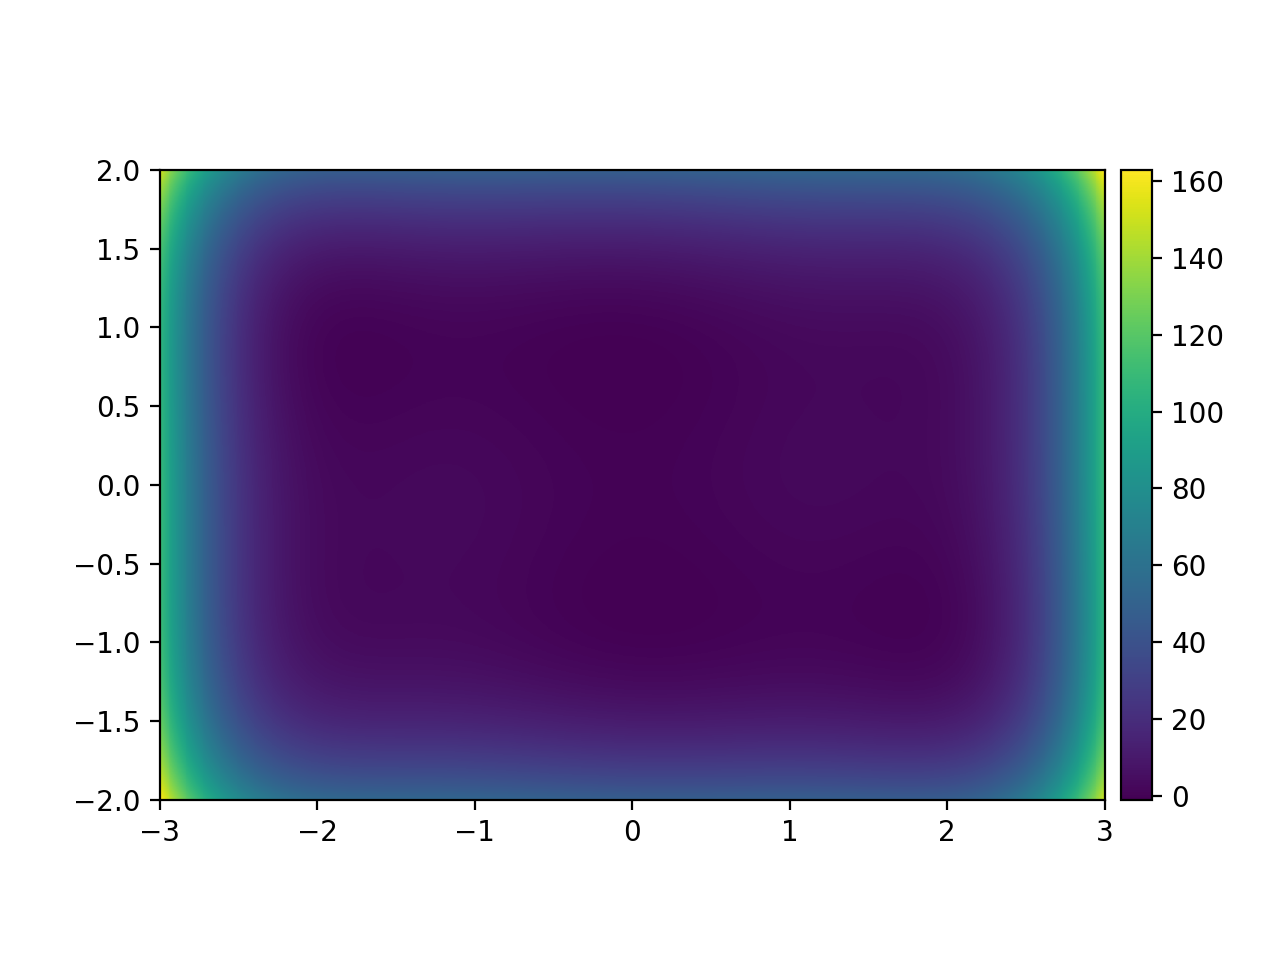
\includegraphics[height=200px]{figures/1_1.png}\end{align*}

\subsection*{2}
This data does not seem stationary. From the heatmap, we can see that the majority of the function away from the boundary are relatively flat compared to regions close to the boundary. That is, the function change drastically when it gets closer to the border of the domain.

\subsection*{3}
Intuitively, we want to apply the logarithm operation to the function value so that values will be transformed clustered to $0$. The most effective region of such behavior is when closer to $0^+$, and non-positive numbers does not have a real logarithm, thus, we applied a linear shift ($-\text{min}+\epsilon$). Such shifted logarithm transformation is applied twice for better behavioral. Specifically, define the transformation as follows,\begin{align}
	\phi(z) = \log(\log(z-\text{min}_1+\epsilon)-\text{min}_2+\epsilon), \\
	\text{min}_1=-1.0279,\ \ \text{min}_2=-0.6931,\ \ \epsilon=0.5.
\end{align}
with the heatmap as follows,
\begin{align*}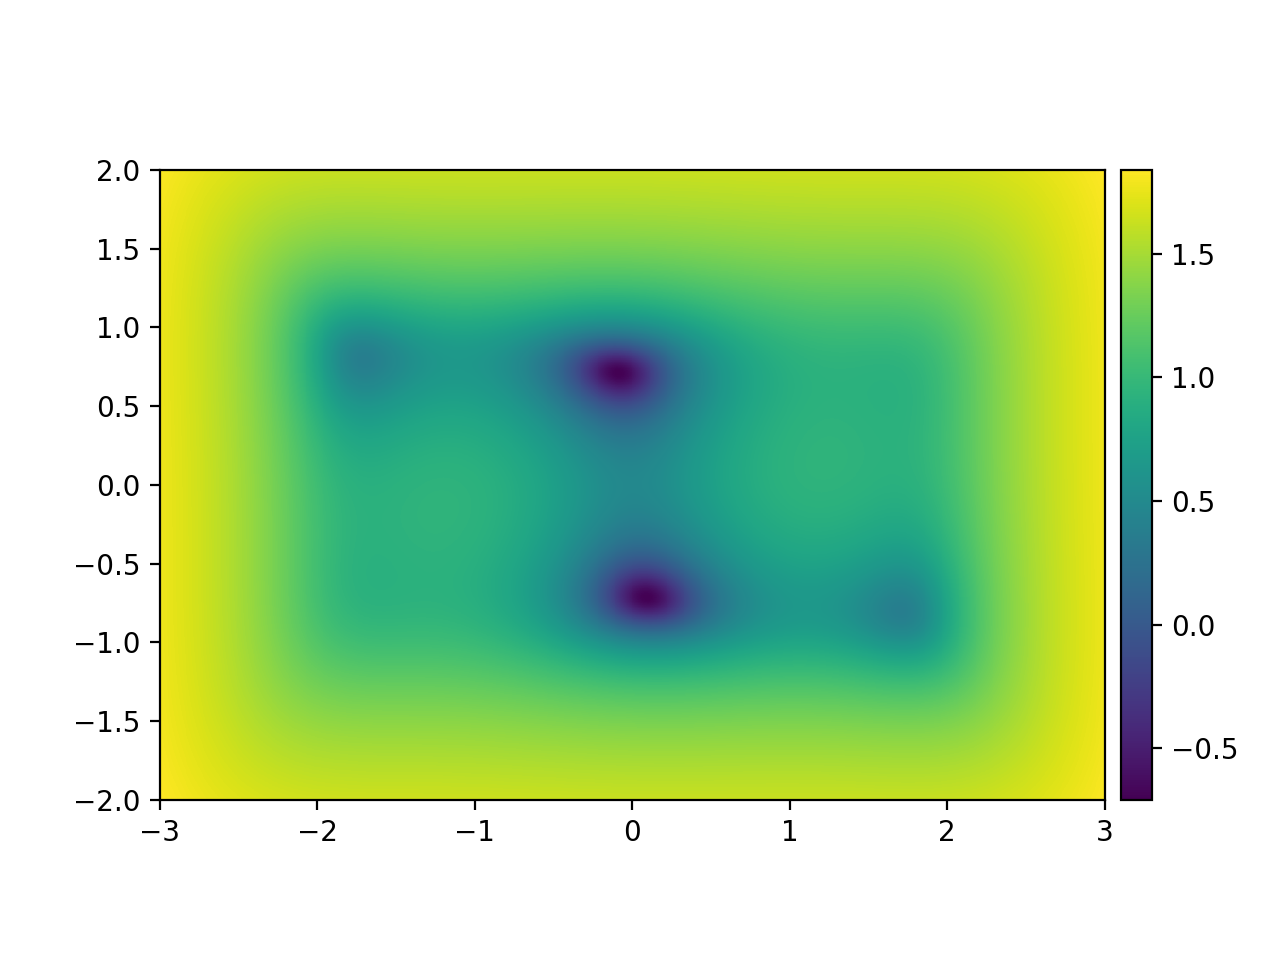
\includegraphics[height=200px]{figures/1_3.png}\end{align*}

\subsection*{4}
Here is the Kernel Density Estimate of $LDA$ and $SVM$,
\begin{align*}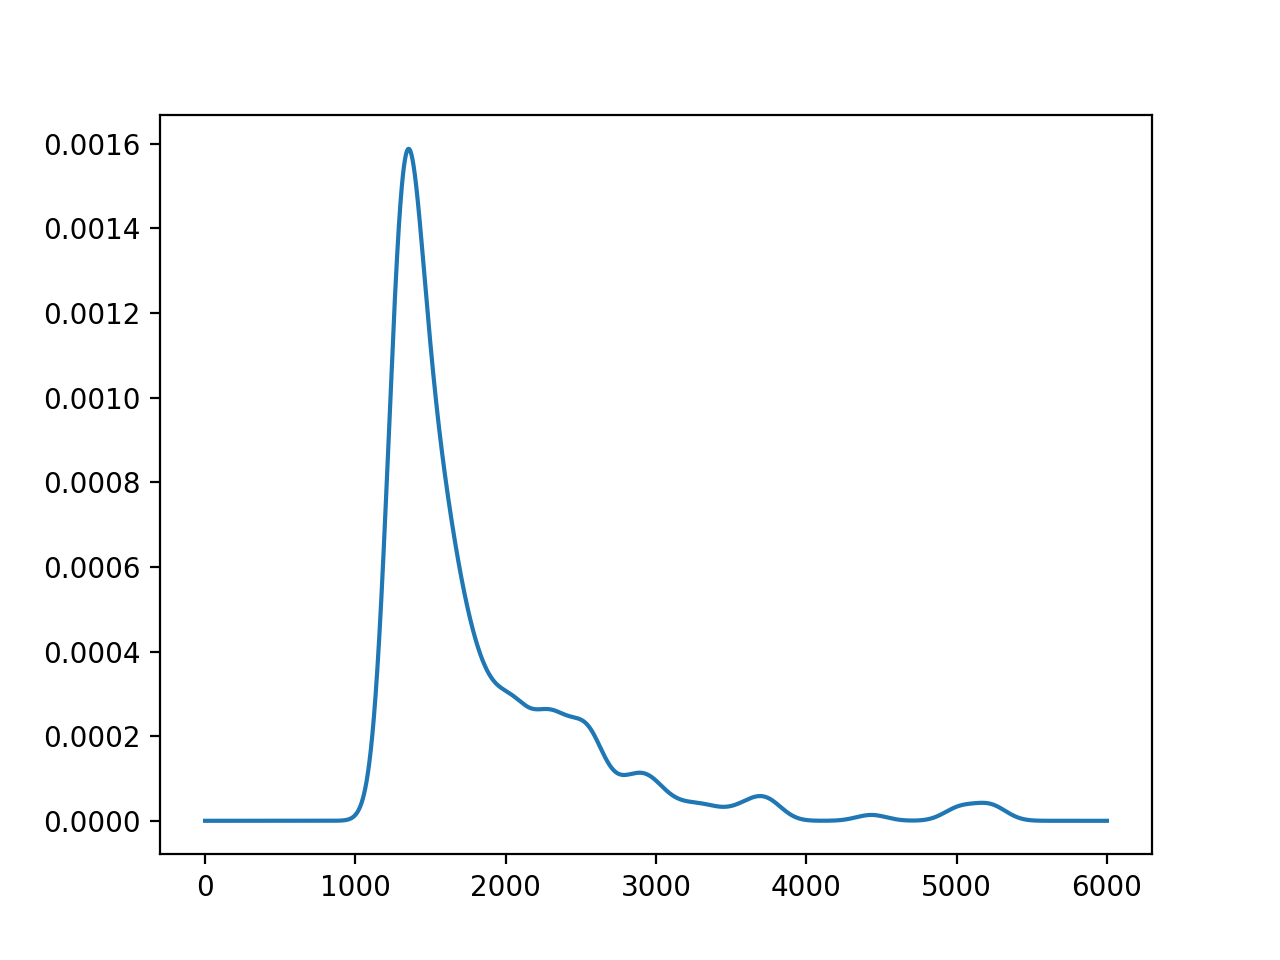
\includegraphics[height=180px]{figures/1_4.1.png}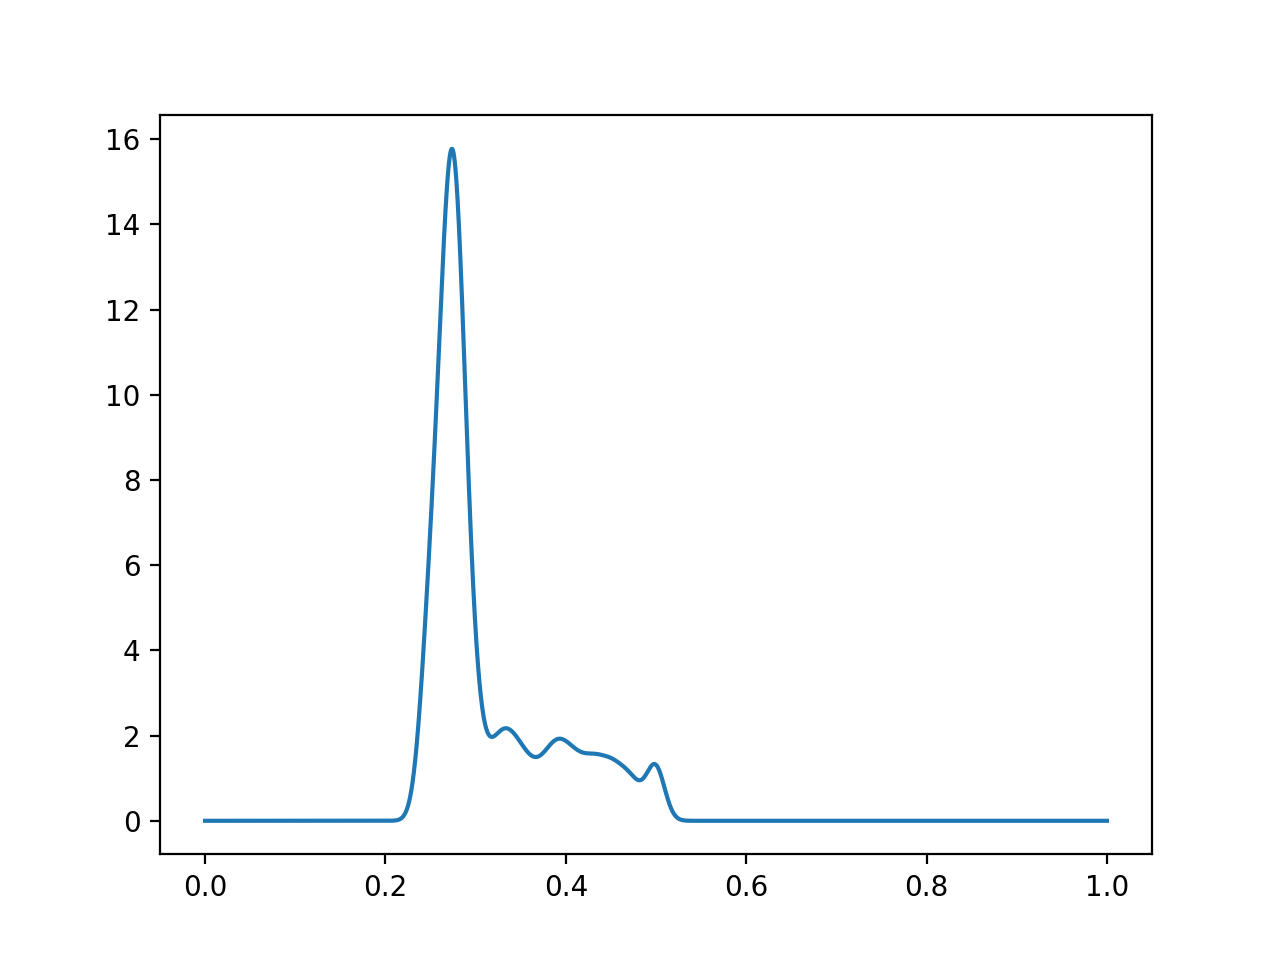
\includegraphics[height=180px]{figures/1_4.2.png}\end{align*}

\subsection*{5}
Here is the Kernel Density Estimate of $LDA$ and $SVM$ after applying $\phi(z)=\log\left(z-1250\right)$ and $\phi(z)=\log\left(z-0.2\right)$,
\begin{align*}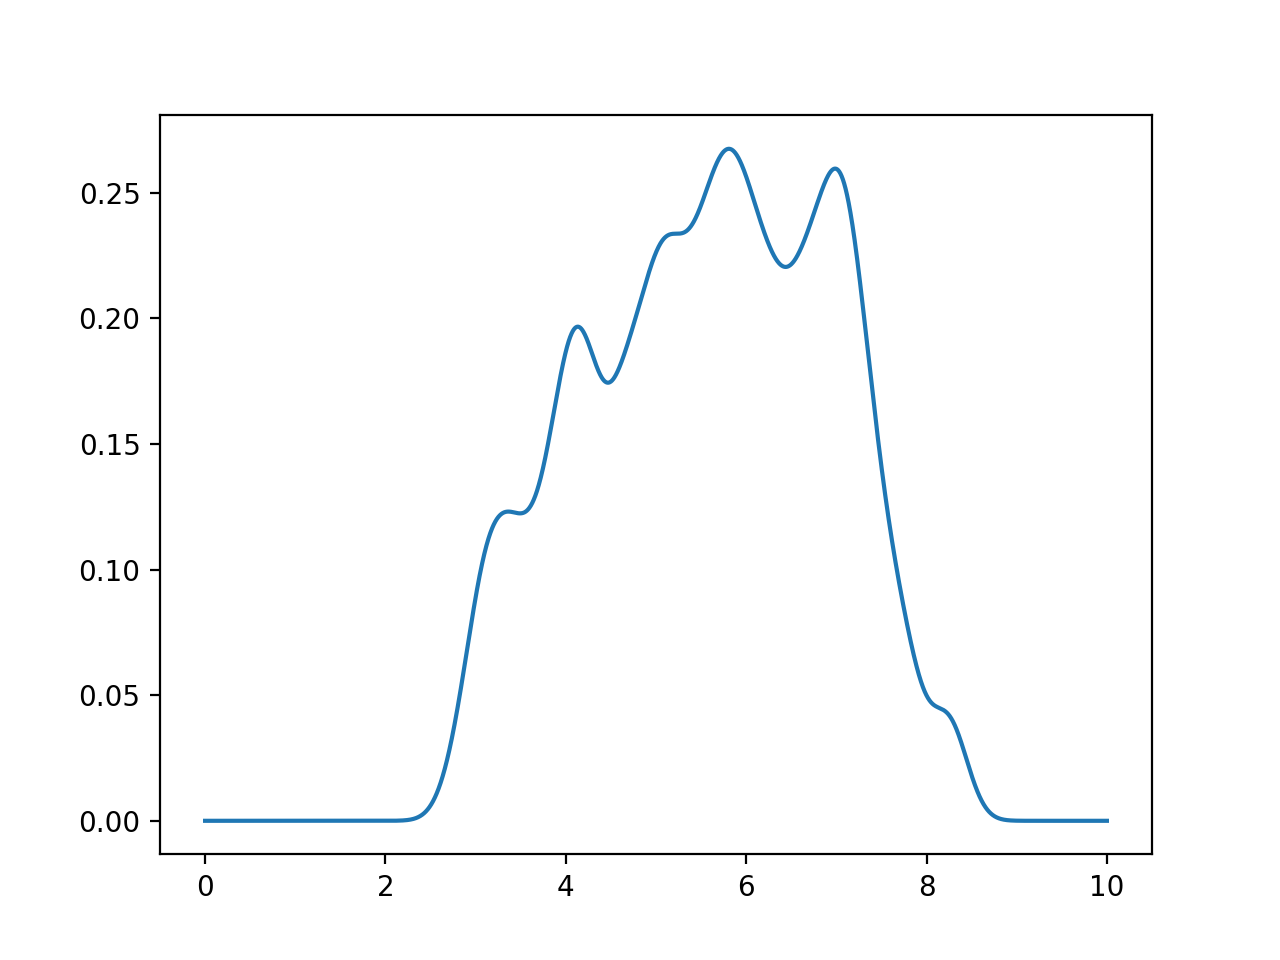
\includegraphics[height=180px]{figures/1_5.1.png}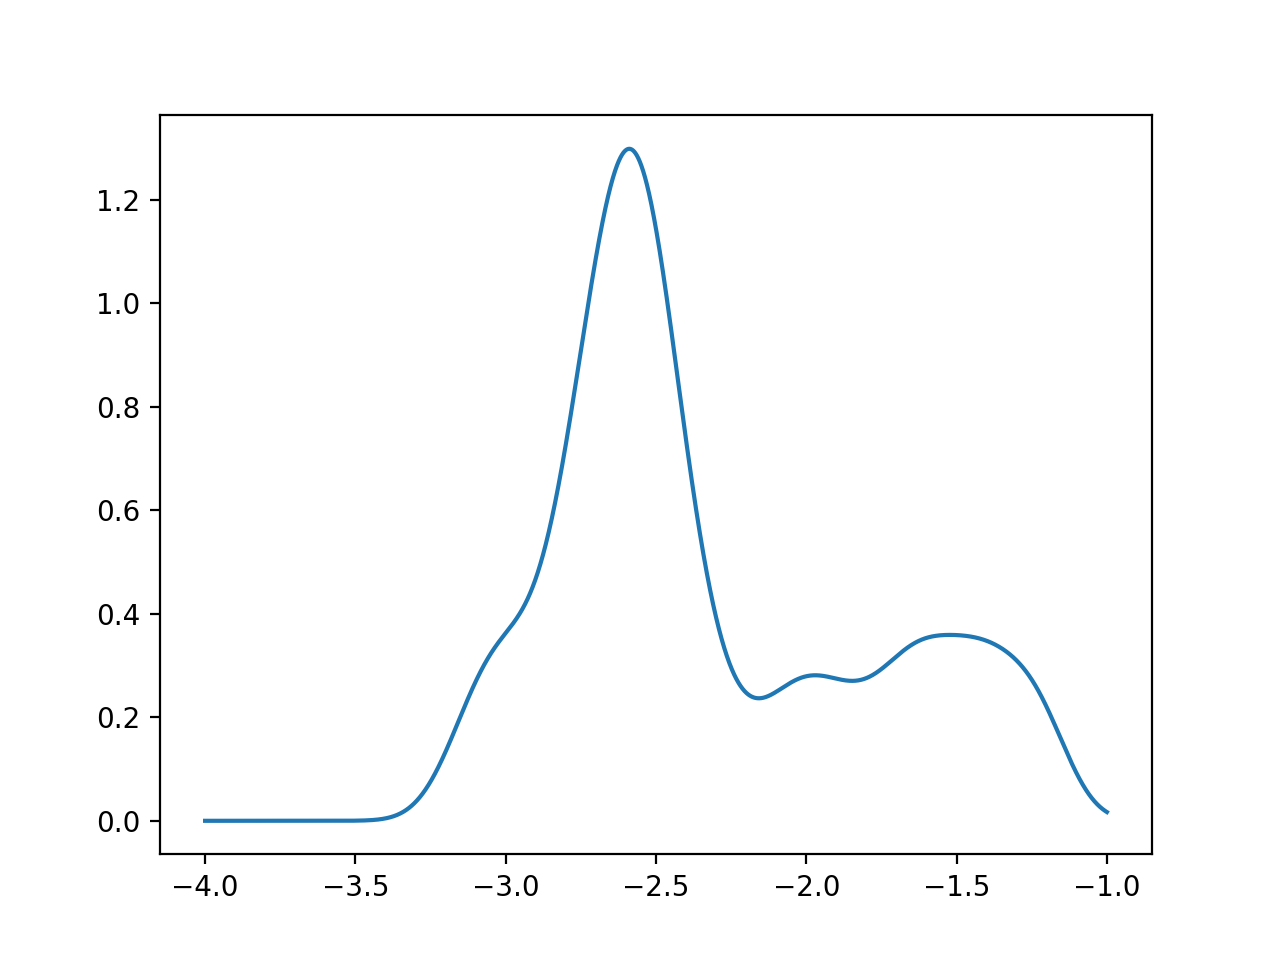
\includegraphics[height=180px]{figures/1_5.2.png}\end{align*}

\newpage
\section{Model Fitting}

\subsection*{Without Transformation}
\subsection*{1}
After picking the Sobol sequence, the function is evaluated, with the height of the marker representing the value of the function.
\begin{align*}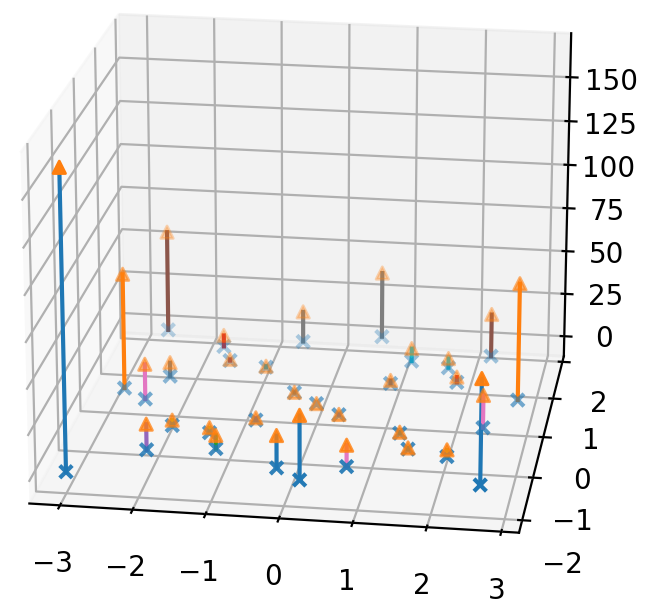
\includegraphics[height=250px]{figures/2_1.png}\end{align*}

\subsection*{2}
After maximizing the log likelihood (which would maximize the likelihood) as a function of the hyperparameters, we reaches a final MLL of $11.0749$ from the initial loss of $-1100.2000$, with the optimal constant mean being optimized from $0$ to $37.8364$, lengthscale from $[0.6931, 0.6931]$ to $[0.5020, 1.3928]$, and output scale from $0.6931$ to $268.1912$.

\subsection*{3}
I agree with all the hyperparameters. \\
In particular, it make sense to have lengthscale of the order around $1$, but with one that is smaller than $1$ and one that is larger. This is because that one the samples we pick from the Sobol sequence, the value changes more on one direction compares to the other. \\
The mean make sense as all the observations are positive, so a mean of $37.8364$ is about correct. The output scale also make sense, it is within the range of the training data, and reasonably closer to the more extreme data in the sample.
\begin{align*}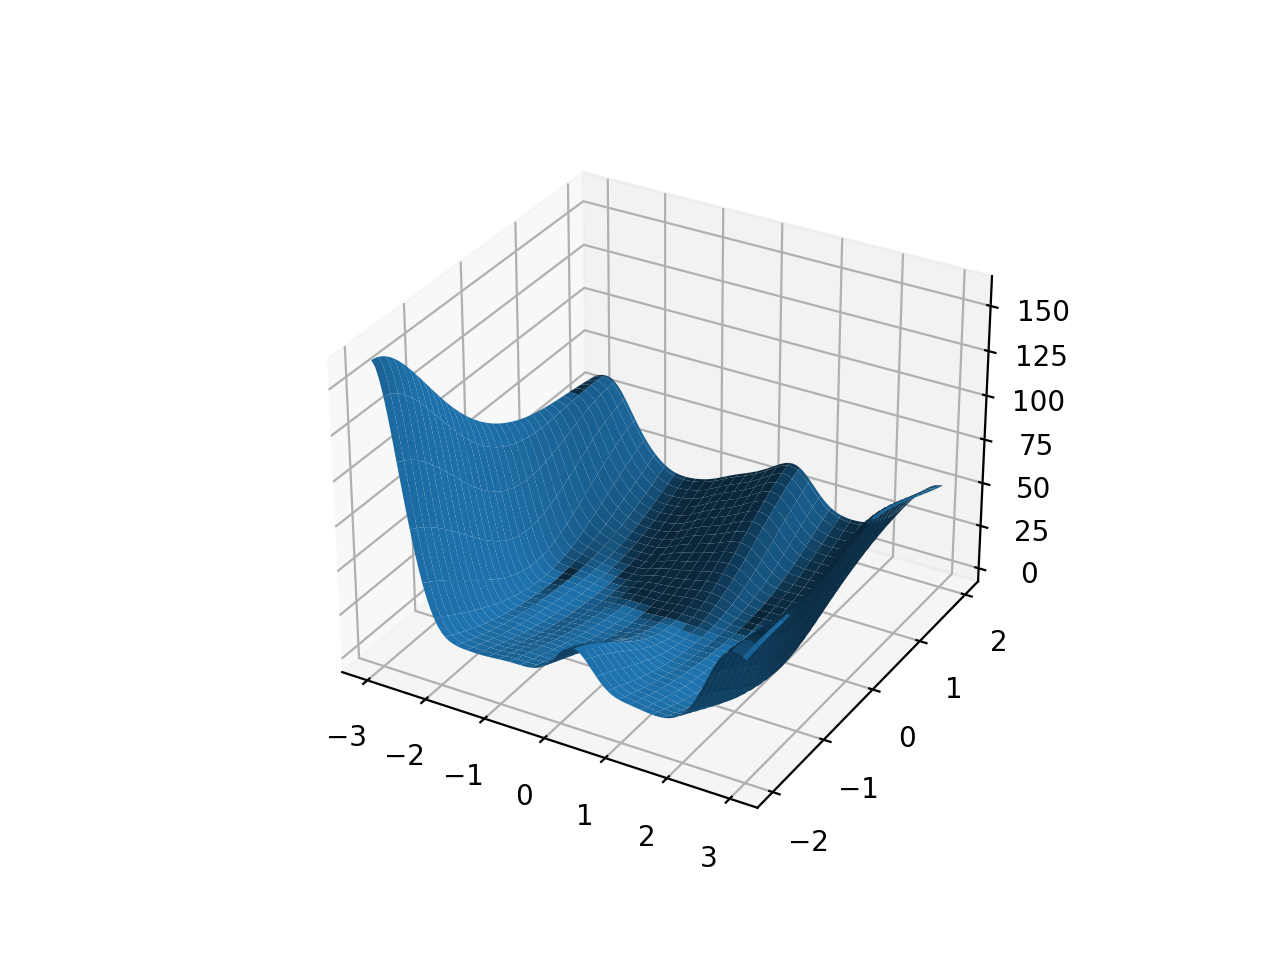
\includegraphics[height=200px]{figures/2_3.png}\end{align*}
Given this visualization of the posterior mean, this is a reasonable Gaussian process at $\mathbb R^2$, and it meets my expectation.

\subsection*{4}
Here is the heatmap of the posterior mean of the Gaussian Process,
\begin{align*}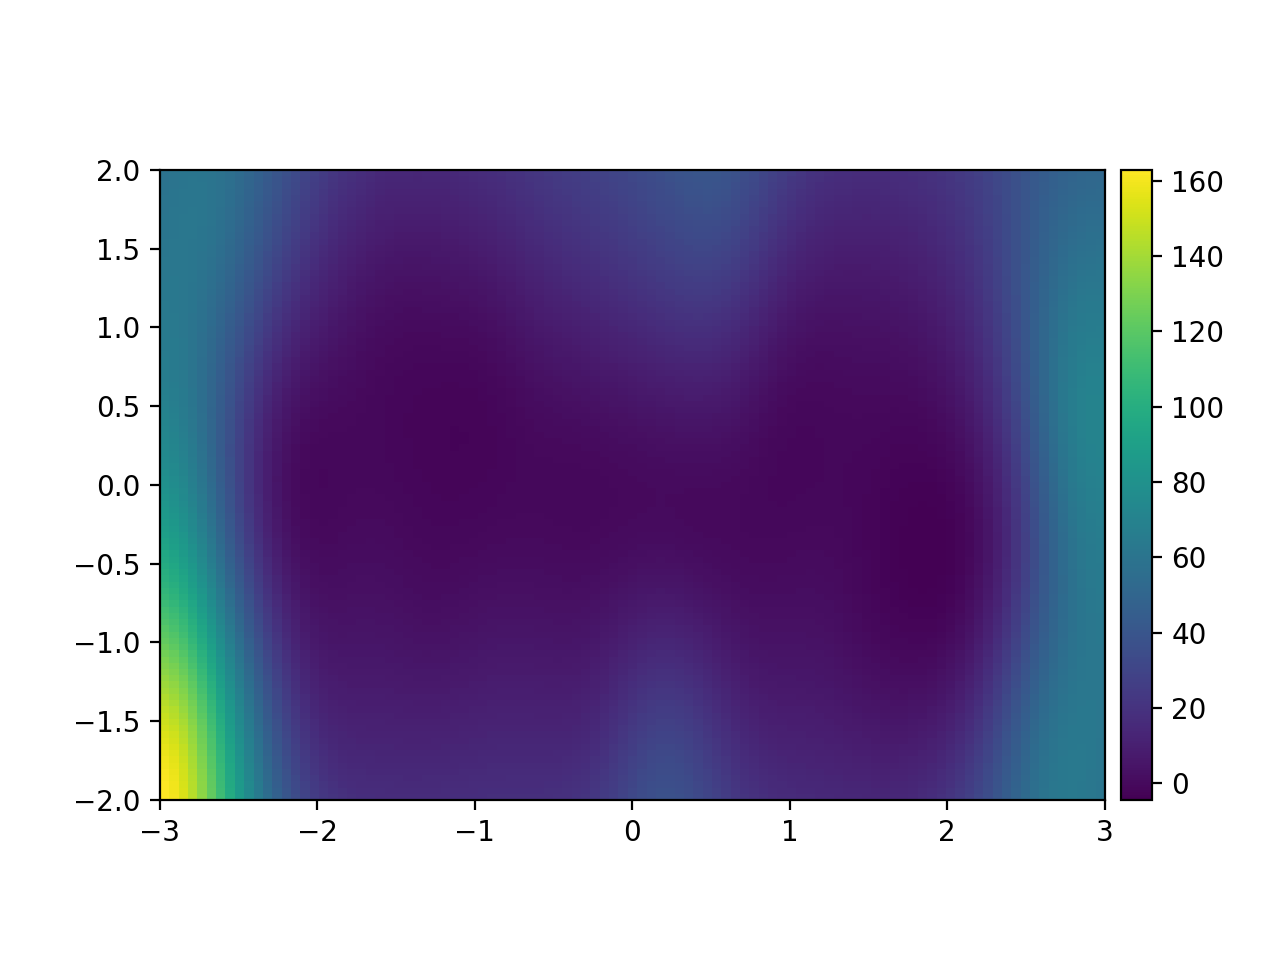
\includegraphics[height=200px]{figures/2_4.1.png}\end{align*}
And here is the absolute difference between the posterior mean and the actual function value,
\begin{align*}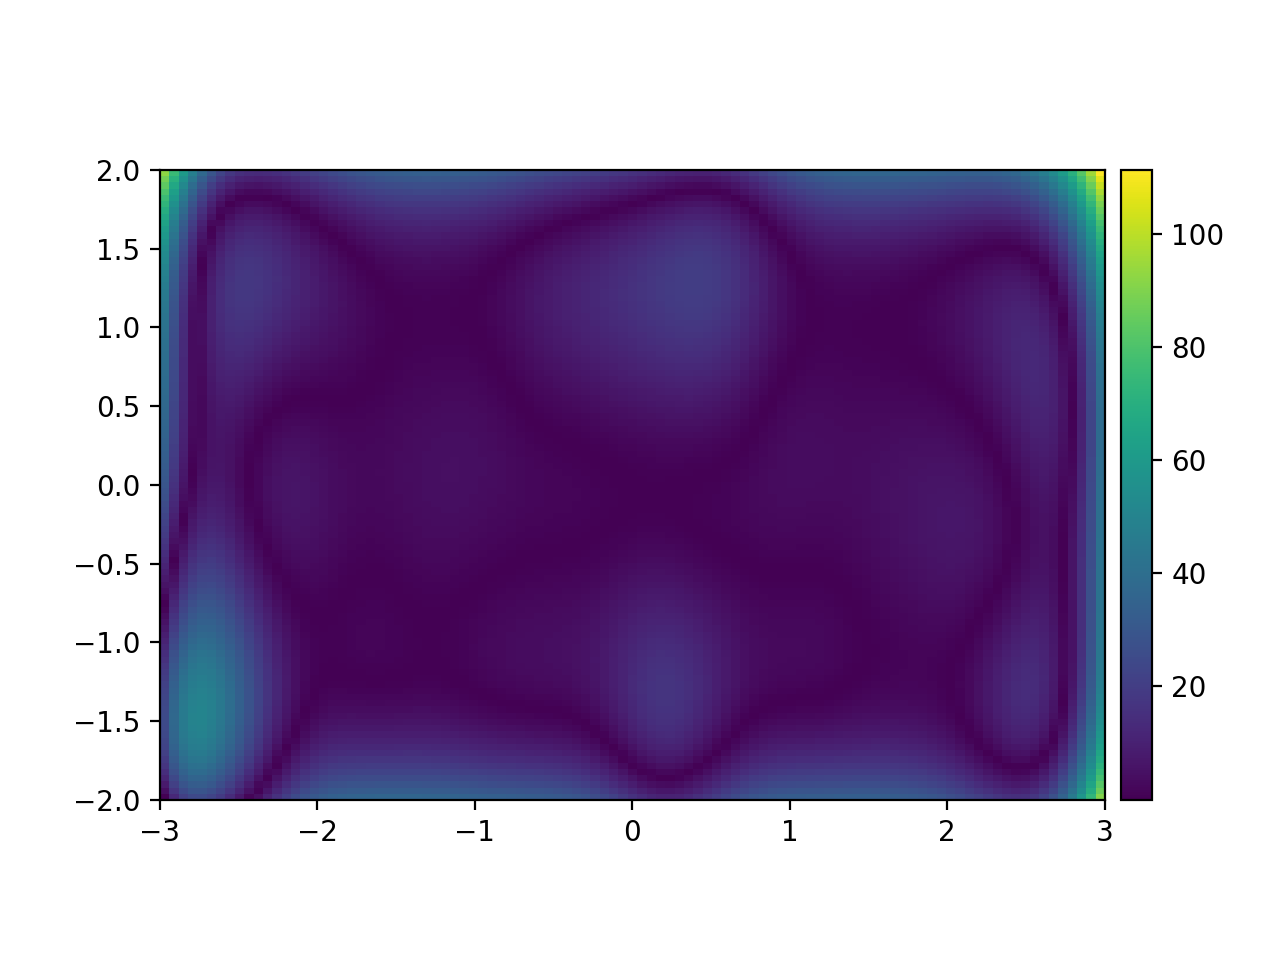
\includegraphics[height=200px]{figures/2_4.2.png}\end{align*}
From the figure, we can see that the heatmap of the posterior mean looks reasonably close to the original function. It appears to be a valid Gaussian process, as the differences almost vanishes at the sampled points, and increases as it moves away from the sampled points.\\
However, after plotting the residue of the posterior mean minus the original function, we realized that there is a systematic error. Specifically, all the posterior mean values are larger than the original function, even though most are relatively close. So, there is a systematic error that all the values are predicted higher than its actual value.
\begin{align*}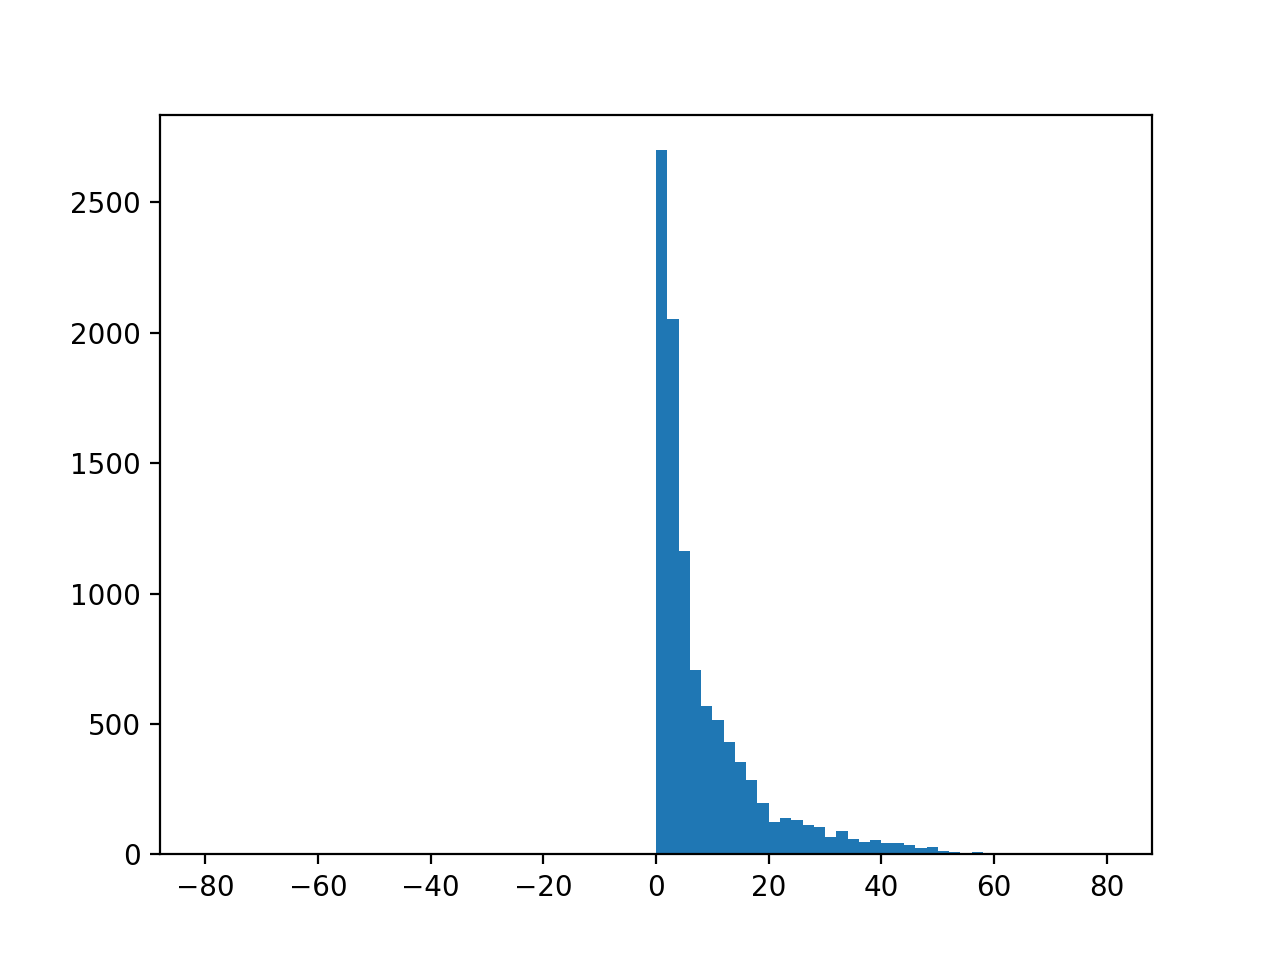
\includegraphics[height=200px]{figures/2_4.3.png}\end{align*}

\subsection*{5}
From the plot, we can see that when closer to the points we sampled for training the Gaussian process, the standard deviation drops to almost zero; and the standard deviation increases as it moves away from sampled locations. Also, since the lengthscale of $x$ is $\leq1$ and the lengthscale of $y$ is $\geq1$, we know that the contours of low standard deviation areas are of ellipsoid shape, stretched on the $x$ direction and shrunk on the $y$ direction. So, in conclusion, this graph of the standard deviation as a function of the domain make sense.
\begin{align*}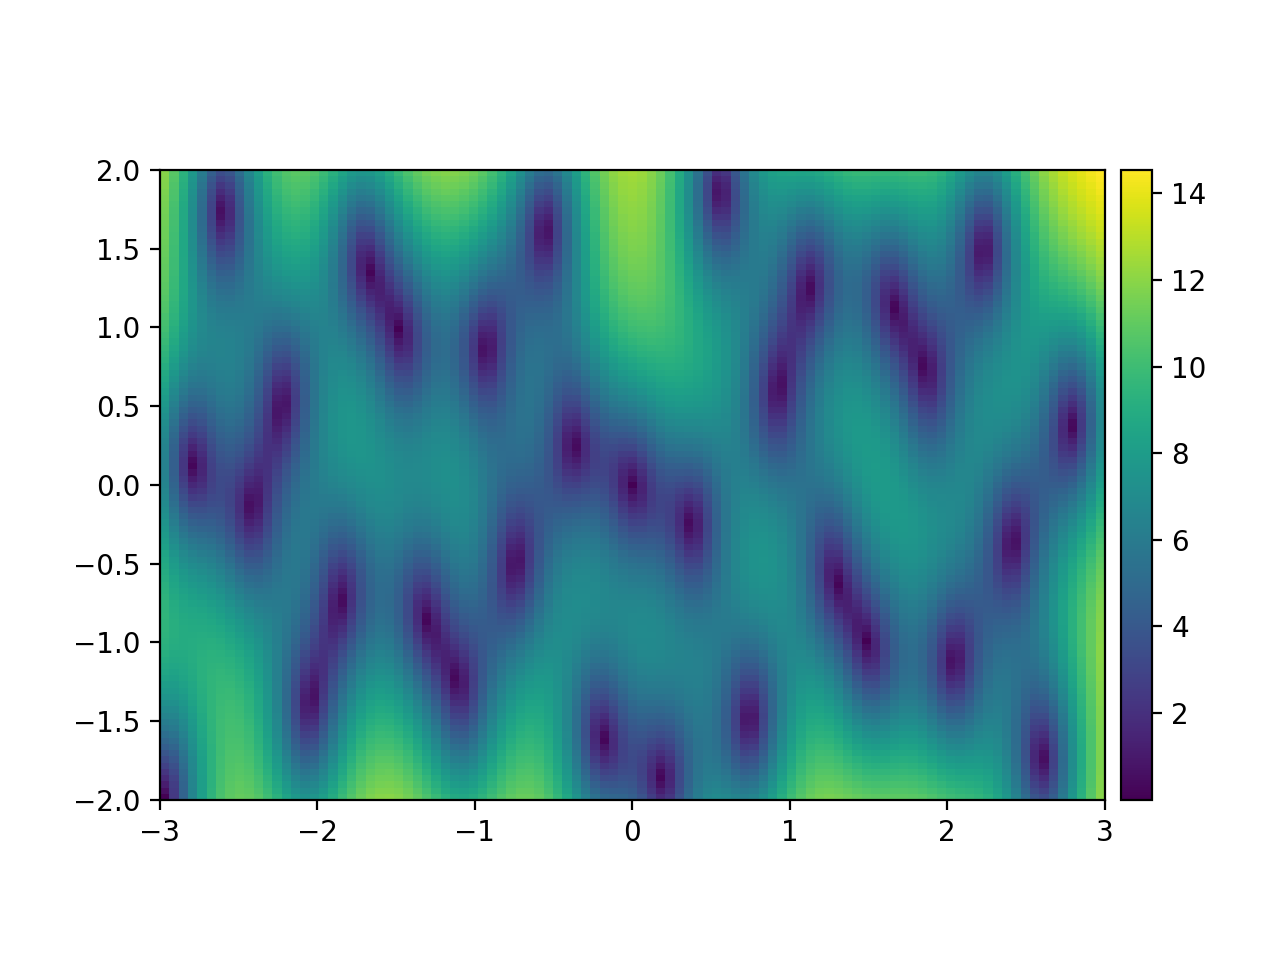
\includegraphics[height=200px]{figures/2_5.png}\end{align*}

\subsection*{6}
From the figure, we can see that (similar to the histogram) our residue are strongly biased. So, this indicates that our model is not well calibrated.
\begin{align*}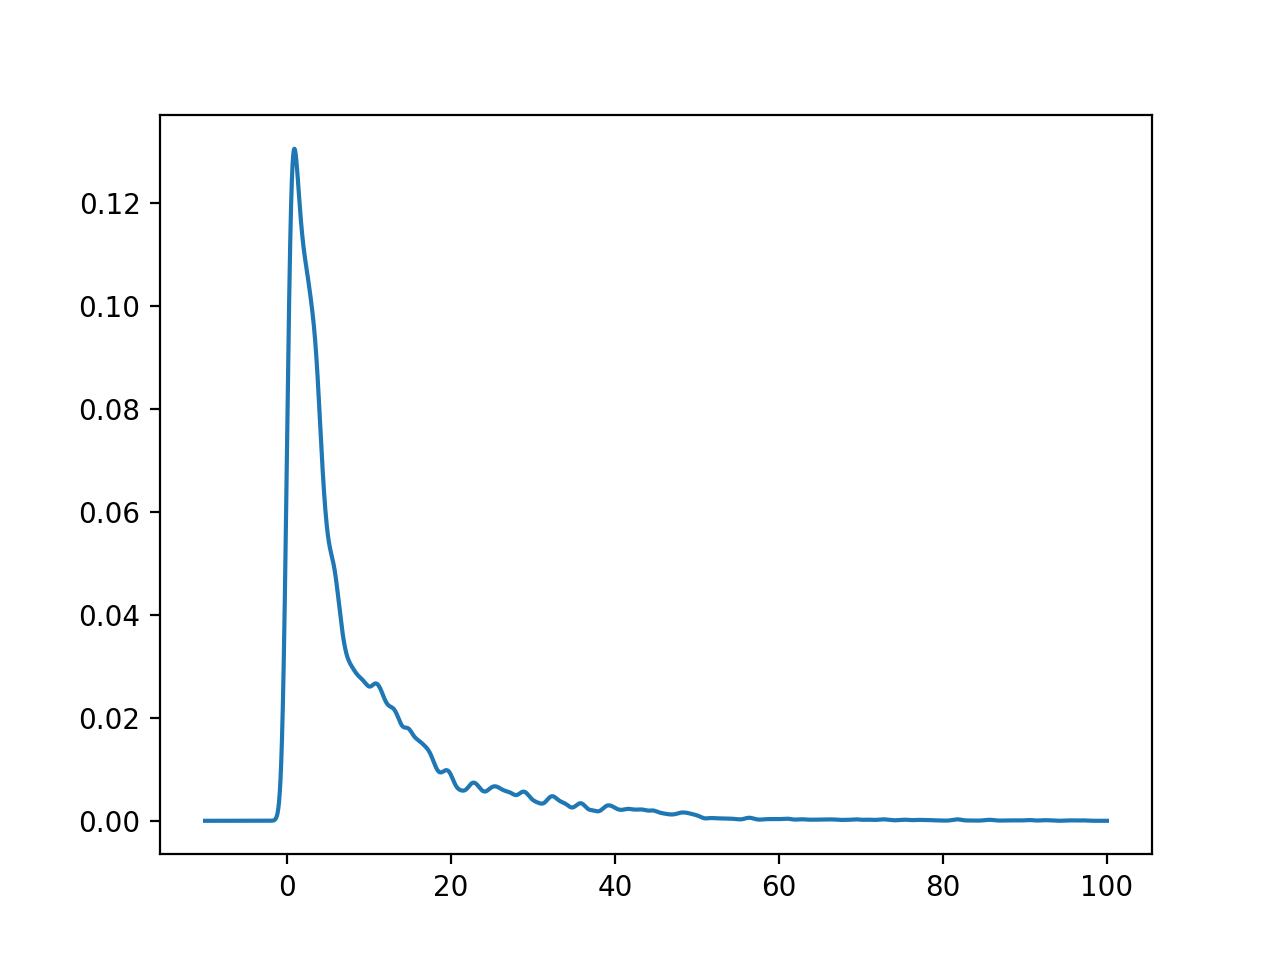
\includegraphics[height=200px]{figures/2_6.png}\end{align*}

\subsection*{With Transformation}
\subsection*{0}
So, in order to make the function nicer, we apply the logarithm function twice to shift the function less skewed. However, since the values might be negative, we also need a small constant term to shift the values. Specifically, denote the $z=f(x)$ be the original output of the six-hump camel function, the formula is given below:
\begin{align}
	\phi(z) = \log(\log(z-\text{min}_1+\epsilon)-\text{min}_2+\epsilon), \\
	\text{min}_1=-1.0279,\ \ \text{min}_2=-0.6931,\ \ \epsilon=0.5.
\end{align}

\subsection*{1}
After picking the same Sobol sequence, the function is evaluated.
\begin{align*}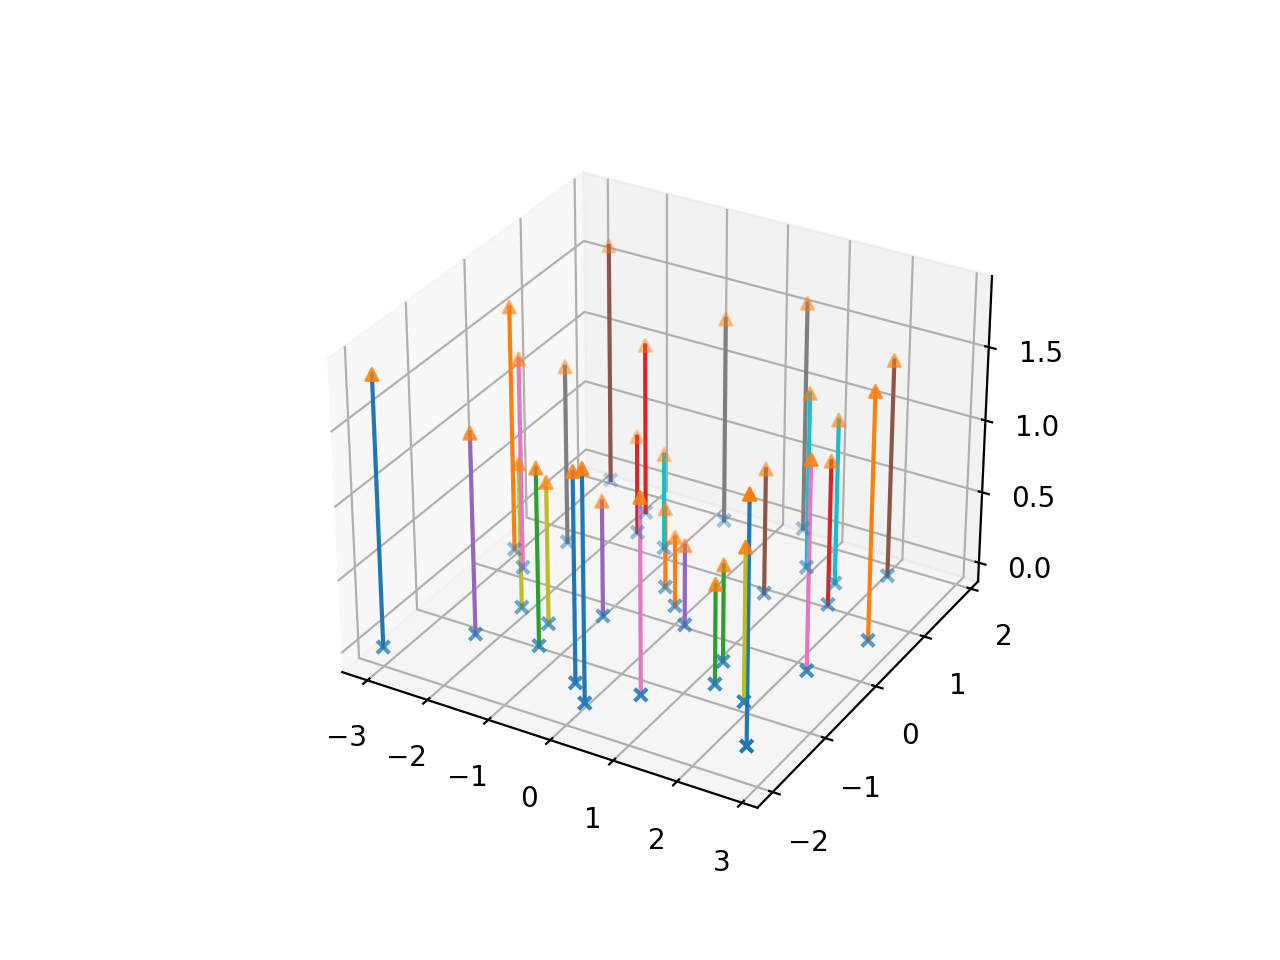
\includegraphics[height=250px]{figures/2_1'.png}\end{align*}

\subsection*{2}
After maximizing the log likelihood (which would maximize the likelihood) as a function of the hyperparameters, we reaches a final loss of $12.0851$ from the initial loss of $-1.3777$, with the optimal constant mean being optimized from $0$ to $1.4924$, lengthscale from $[0.6931, 0.6931]$ to $[1.1967, 0.9132]$, and output scale from $0.6931$ to $0.1446$.

\subsection*{3}
I agree with all the hyperparameters. In particular, it make sense to have lengthscale of the order around $1$. The constant mean function $1.4924$ and the output scale $0.6931$ are about correct as the mean is about the average of the function within the domain and the output scale is small.
\begin{align*}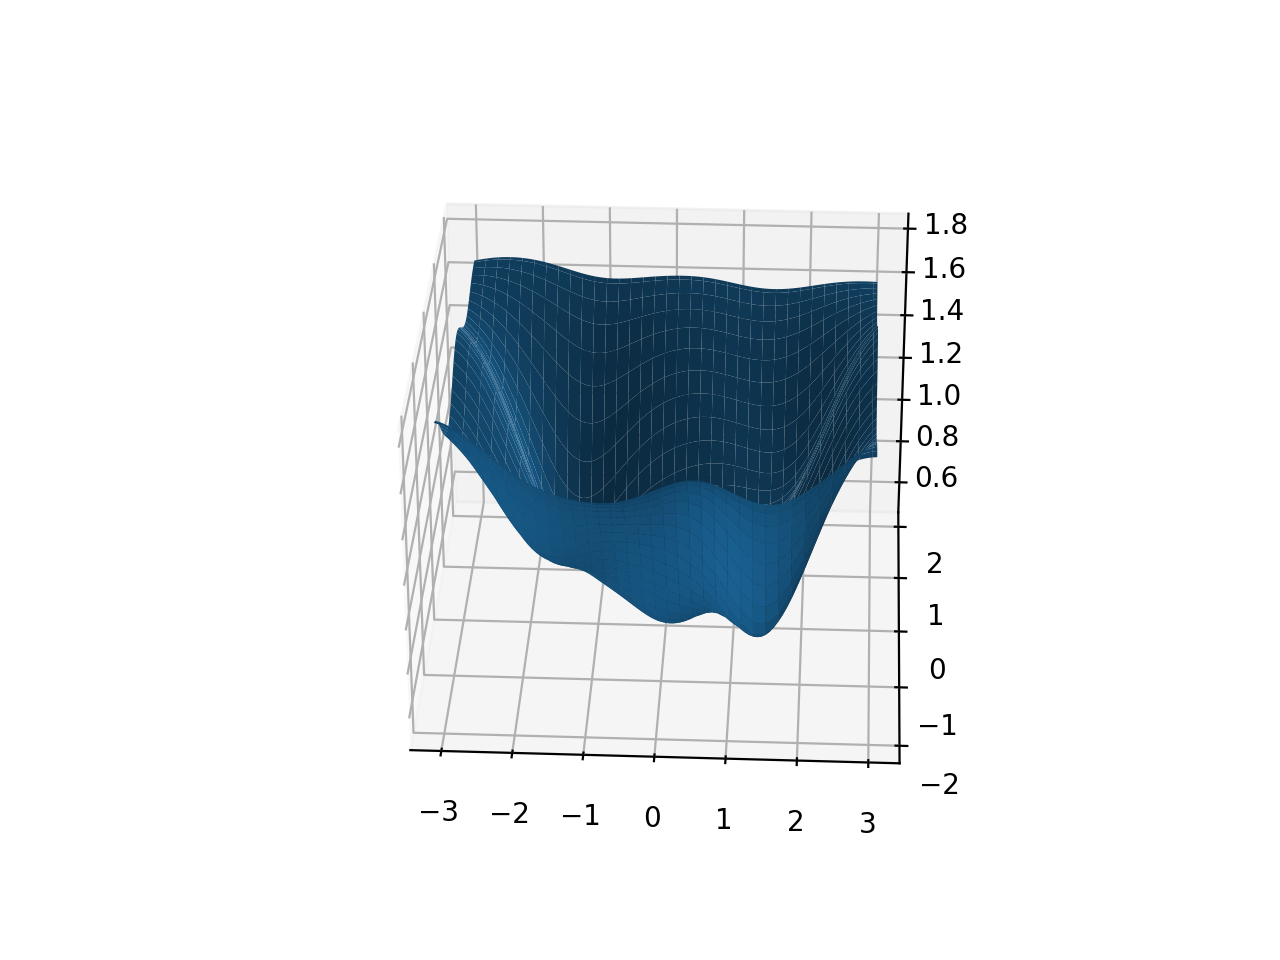
\includegraphics[height=200px]{figures/2_3'.png}\end{align*}
Given this visualization of the posterior mean, this is a reasonable Gaussian process at $\mathbb R^2$, and it meets my expectation.

\subsection*{4}
Here is the heatmap of the posterior mean of the Gaussian Process,
\begin{align*}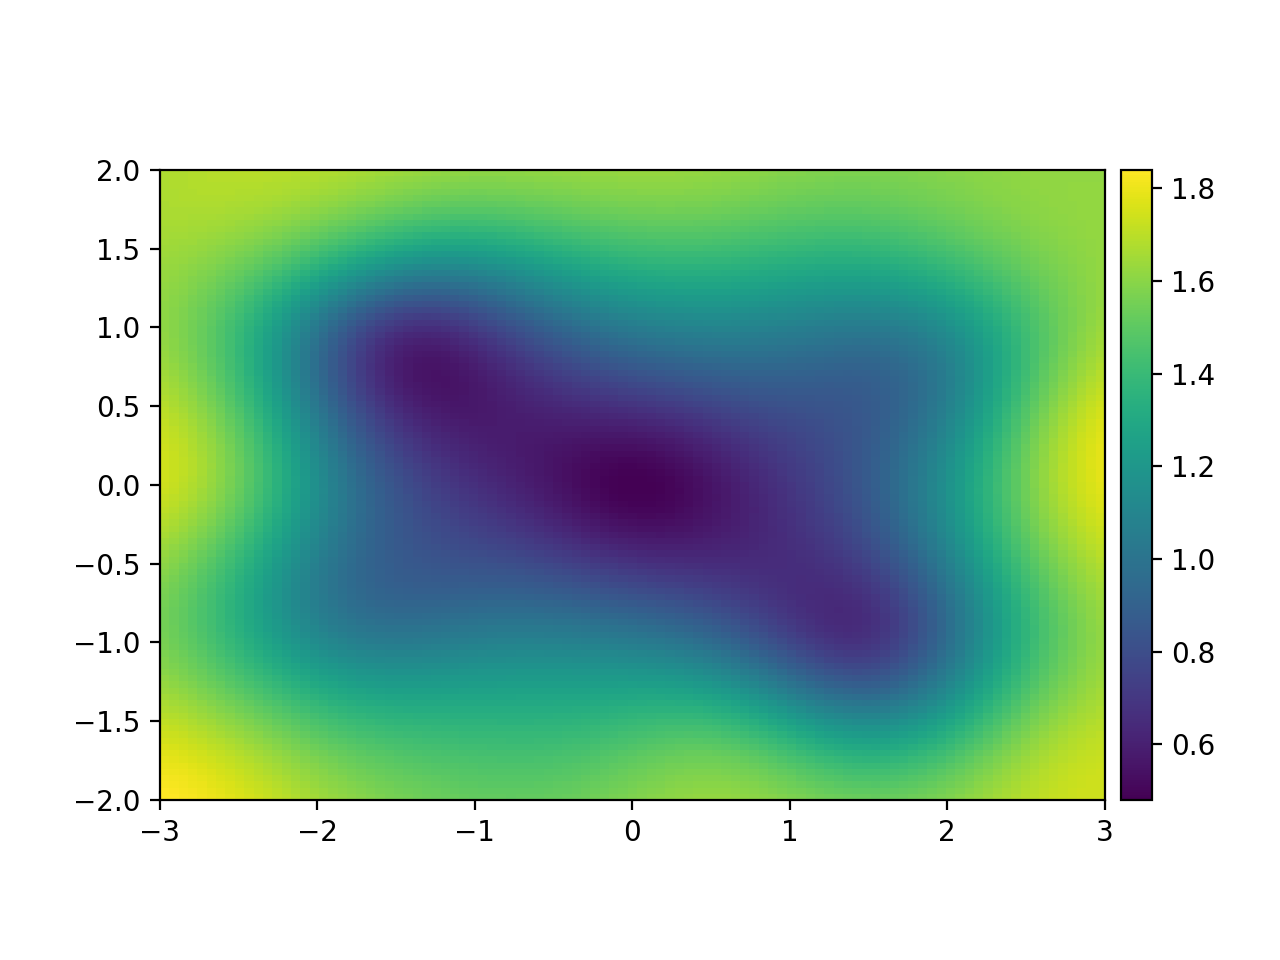
\includegraphics[height=200px]{figures/2_4.1'.png}\end{align*}
And here is the absolute difference between the posterior mean and the actual function value,
\begin{align*}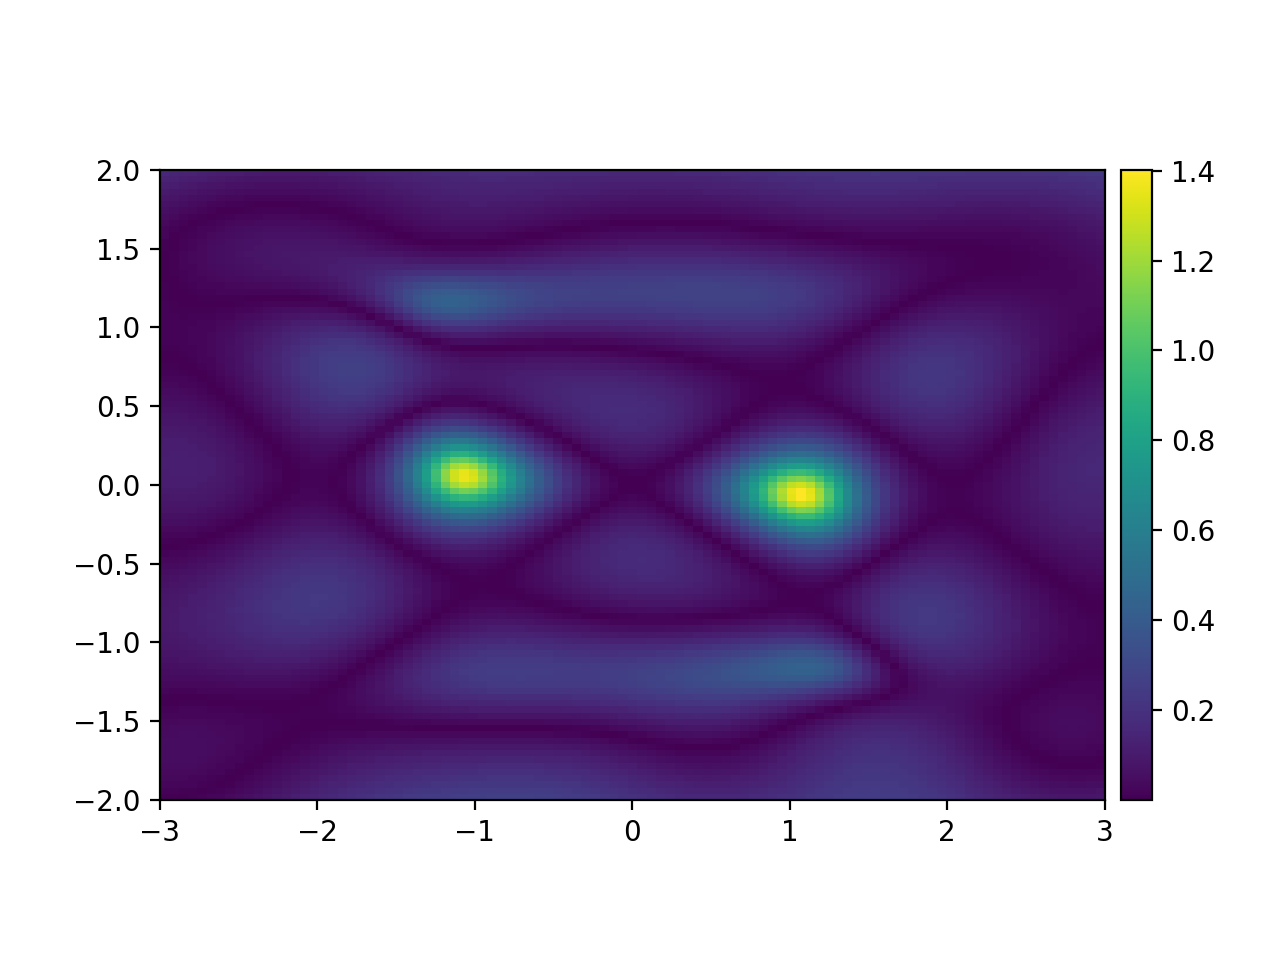
\includegraphics[height=200px]{figures/2_4.2'.png}\end{align*}
From the figure, we can see that the heatmap of the posterior mean looks reasonably close to the original function. It appears to be a valid Gaussian process, as the differences almost vanishes at the sampled points, and increases as it moves away from the sampled points. And there is still a small systematic error, as the residuals are still mostly positive.

\subsection*{5}
From the plot, we see that standard deviation drops to almost zero when closer to the samples used for training. The contours of low standard deviation areas are ellipse of a reasonable ration between axes. So, in conclusion, this graph make sense.
\begin{align*}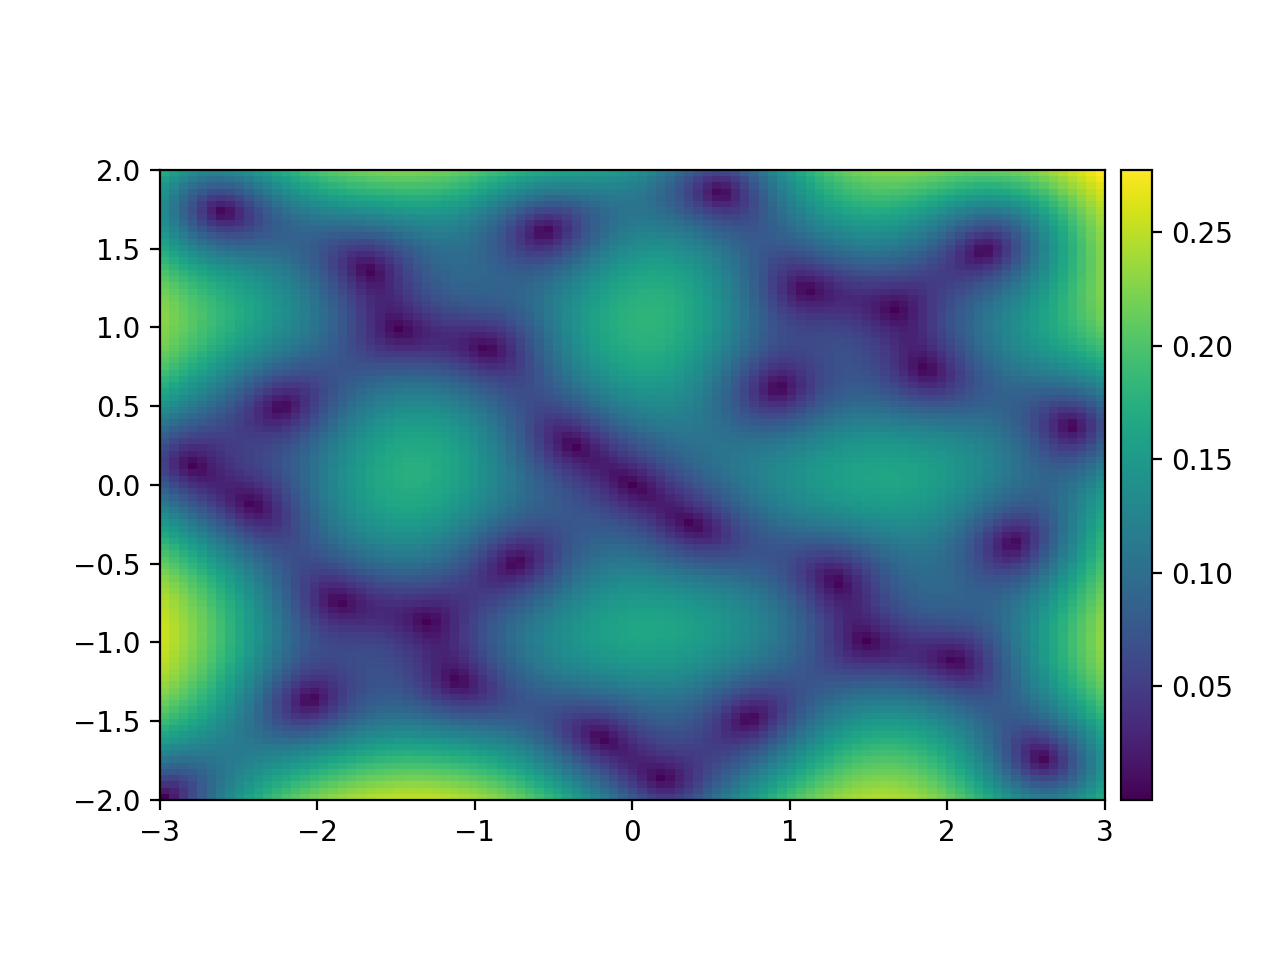
\includegraphics[height=200px]{figures/2_5'.png}\end{align*}

\subsection*{6}
From the figure, we can see that the kernel density estimate of the residuals are more normal than what was before. 
\begin{align*}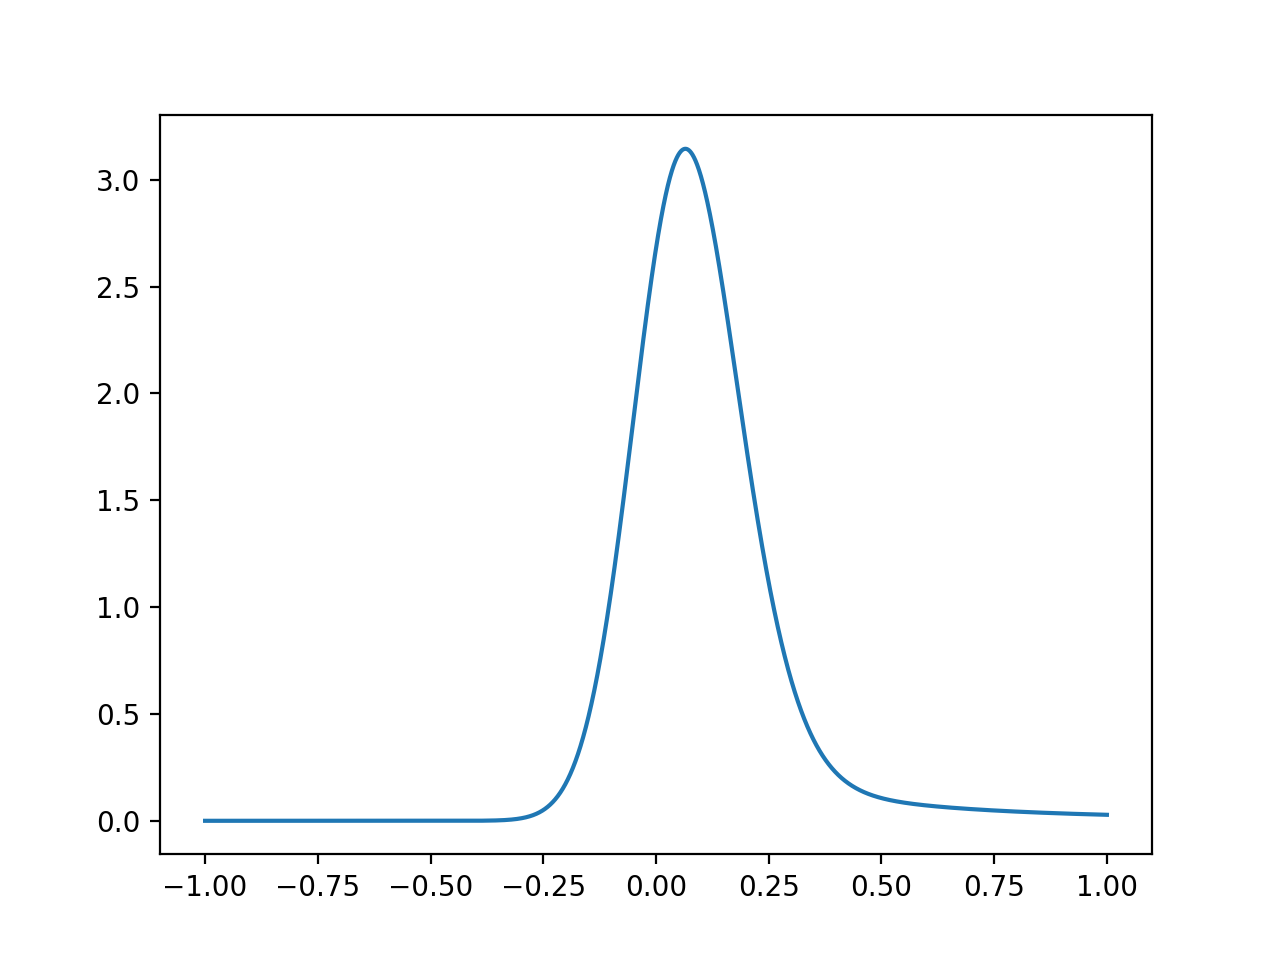
\includegraphics[height=200px]{figures/2_6'.png}\end{align*}

\subsection*{BIC}
\subsection*{1}
The model in the previous part has a BIC score optimized from $13.8989$ to $-14.3271$, with constant mean $1.8050$ and Matérn $\mu=2.5$.

\subsection*{2}
The BIC score was optimized from $12.6163$ to $-14.3272$ with constant mean $1.4582$ and square-exponential covariance; from $13.8989$ to $-14.3271$ constant mean $1.8050$ and Matérn $\mu=2.5$; from $12.9848$ to $-14.3272$ constant mean $2.0995$ and Matérn $\mu=1.5$; from $13.1506$ to $-13.7403$ constant mean $2.1153$ and Matérn $\mu=0.5$.\\
So, the best model (from the $5$th digit after decimal) is the one with constant mean $1.4582$ and square-exponential covariance kernel.

\subsection*{3}
For the LDA data, after applying the transformation proposed in $1.5$, we have the following result:

\begin{center}
\begin{tabular}{|c|c|c|c|}
\hline
$\mu$ & $K$ & $BIC_0$ & $BIC^*$ \\ 
\hline
\hline
$\mu=5.3734$ & $K_{SE}$ & $39.0419$ & $-14.3272$ \\ 
\hline
$\mu=5.3641$ & $K_{M_{0.5}}$ & $39.1948$ & $-12.0864$ \\ 
\hline
$\mu=5.3717$ & $K_{M_{1.5}}$ & $38.8442$ & $-14.0143$ \\ 
\hline
$\mu=5.3724$ & $K_{M_{2.5}}$ & $38.8720$ & $-14.3272$ \\ 
\hline
\end{tabular}
\end{center}

For the SVM data, after applying the transformation proposed in $1.5$, we have the following result:

\begin{center}
\begin{tabular}{|c|c|c|c|}
\hline
$\mu$ & $K$ & $BIC_0$ & $BIC^*$ \\ 
\hline
\hline
$\mu=-2.2951$ & $K_{SE}$ & $16.6320$ & $-14.3272$ \\ 
\hline
$\mu=-2.4698$ & $K_{M_{0.5}}$ & $17.0852$ & $-5.8099$ \\ 
\hline
$\mu=-2.3574$ & $K_{M_{1.5}}$ & $16.8240$ & $-14.3272$ \\ 
\hline
$\mu=-2.3105$ & $K_{M_{2.5}}$ & $16.7430$ & $-3.5101$ \\ 
\hline
\end{tabular}
\end{center}

So, from the observation, we know that constant mean $\mu=5.3734$ with  Matérn $2.5$ is the best model for the LDA dataset, and the constant mean $\mu=-2.3574$ with square-exponential kernel is the best model ($5th$ digit after decimal) for the SVM dataset.

\newpage

\section{Bayesian Optimization}

\subsection*{1}
As instructed, the function for the expected improvement is in the file \textit{main3\_bayesopt1\_hump.py} on line $51$ (begin with \textit{def EI(...)}). Parameters are \textit{numpy} arrays indicating the means, standard deviations, and the current optimal function value.

\subsection*{2}
First, we negate the objective function, i.e., all the function values are now $\phi = - \phi_0$, so that maximizing the new objective function would be equivalent to minimizing the original. Here are the heatmaps for the posterior mean and standard deviation of the domain given the $32$ samples, as well as the heatmap for the expected improvement function, with the maximum location being marked.
\begin{align*}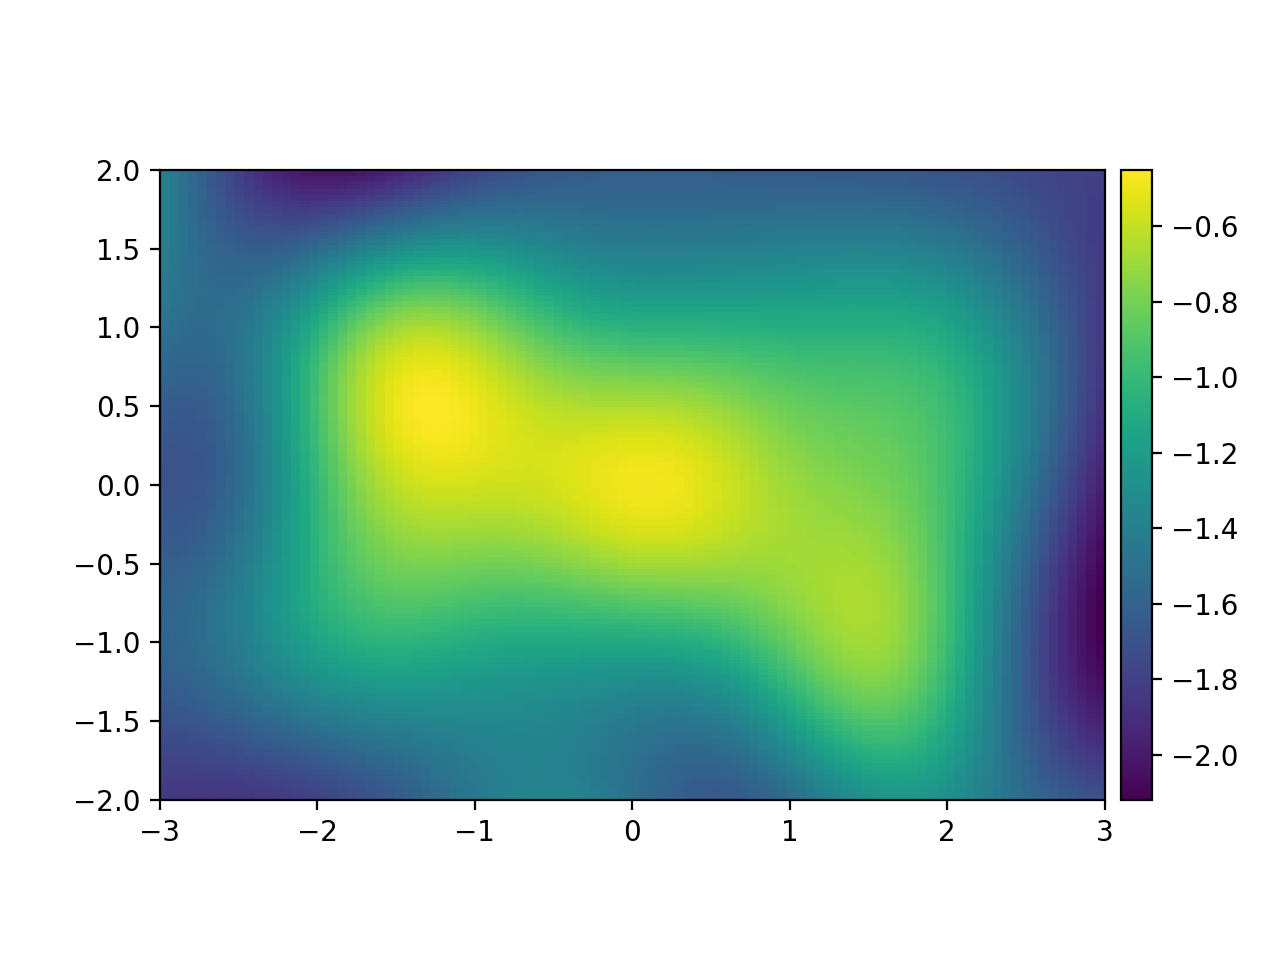
\includegraphics[height=200px]{figures/3_2.1.png}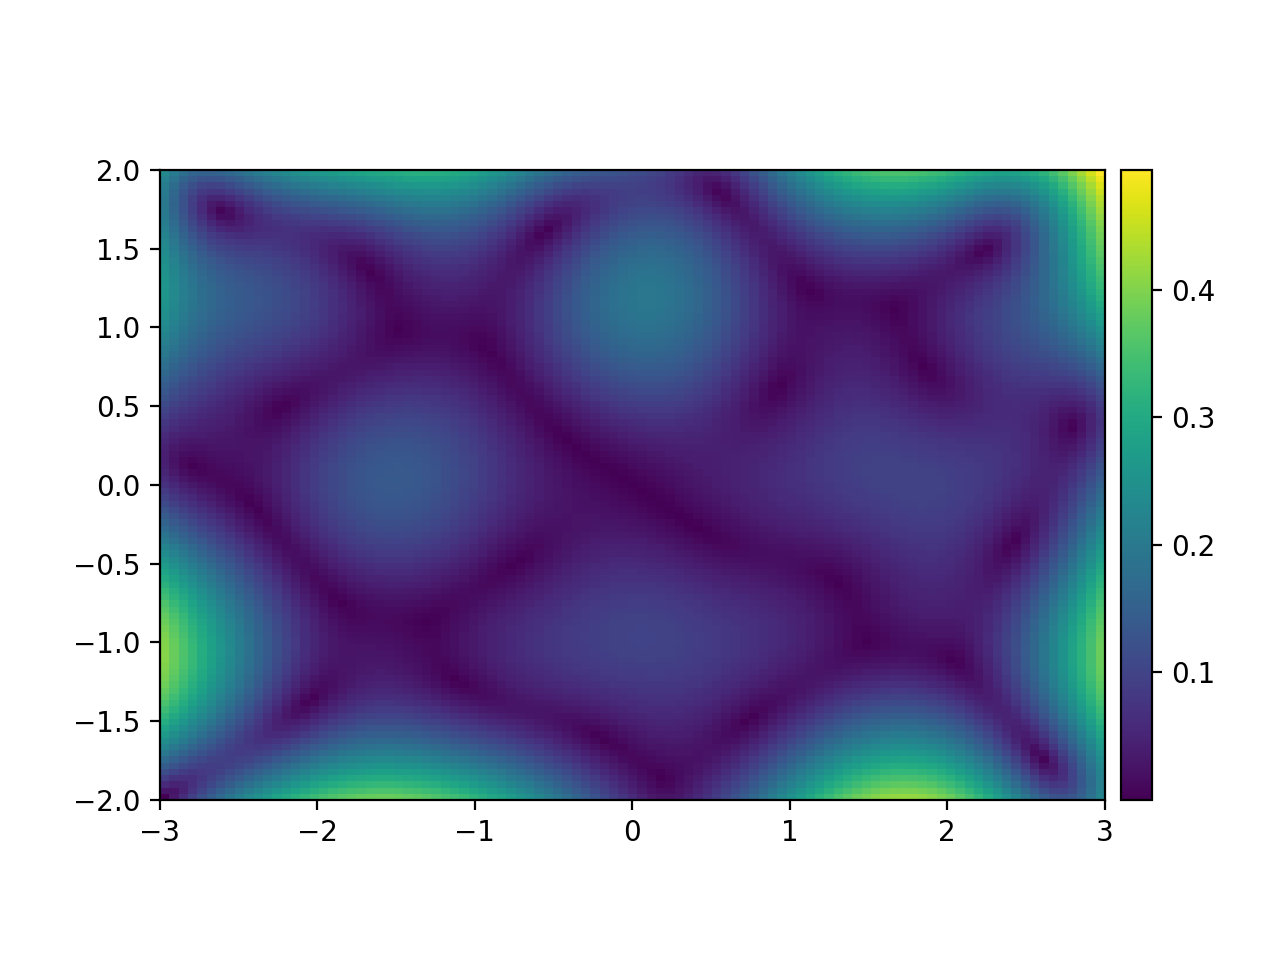
\includegraphics[height=200px]{figures/3_2.2.png}\end{align*}
\begin{align*}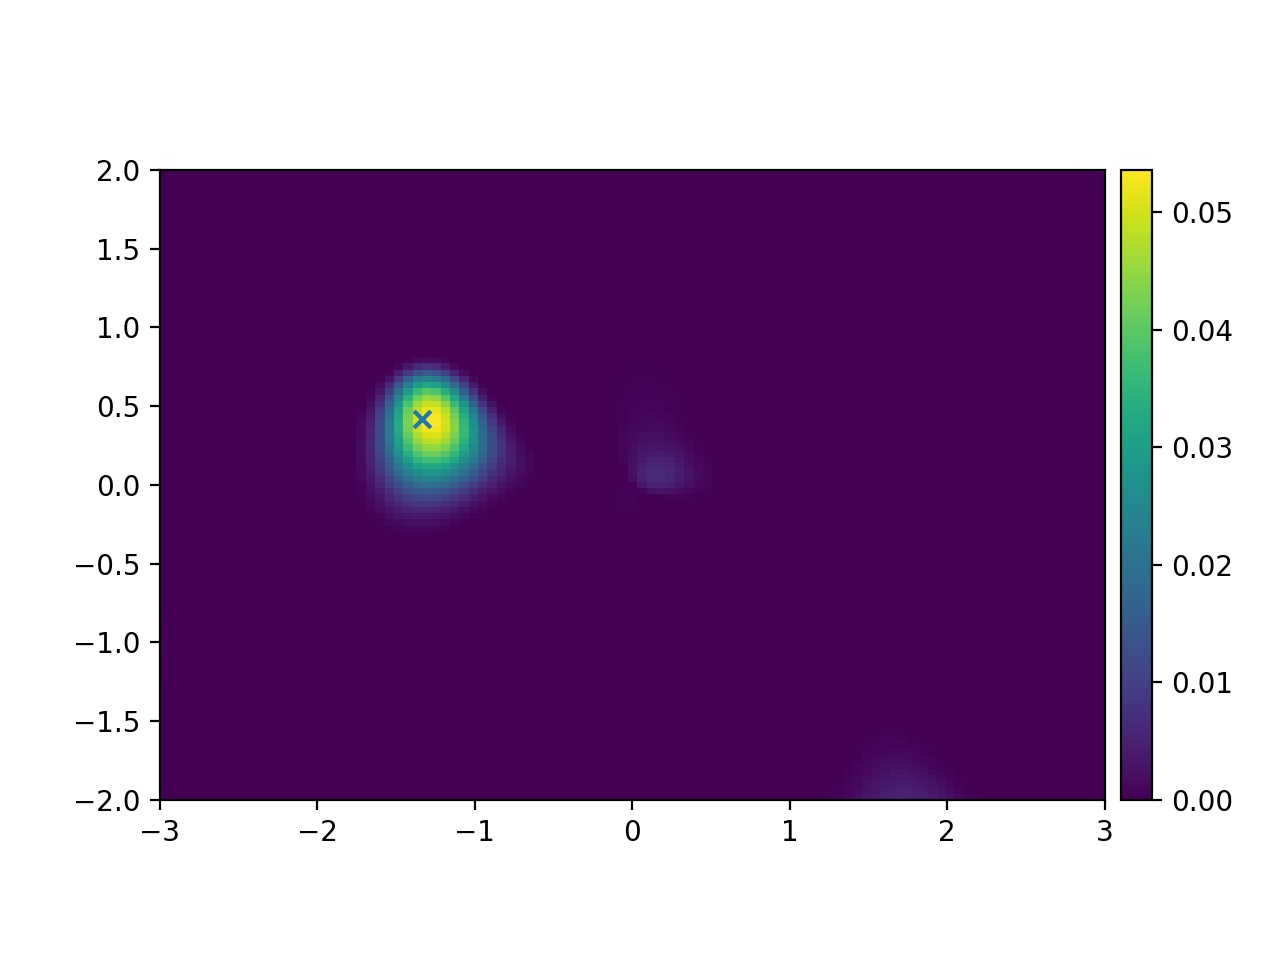
\includegraphics[height=200px]{figures/3_2.3.png}\end{align*}
Clearly, we can see that the location with the maximum expected improvement is on a region with relatively high posterior mean and high posterior standard deviation. This seems to be a good next observation location, as locations with high posterior means and standard deviations are more likely to yield higher observations and functions values.

\subsection*{3}
As it is written in the file \textit{main3\_bayesopt2\_hump.py} and \textit{main3\_bayesopt2\_lda\_svm.py}.

\subsection*{4}
As the gap function being implemented as \textit{gap} in \textit{main3\_bayesopt2\_hump.py} for the six-hump function and \textit{main3\_bayesopt2\_lda\_svm.py} for the LDA and SVM dataset.

\subsection*{5}
The experiments are run in the same file.

\subsection*{6}
Here are the learning curves of the three problem (six-hump, LDA, SVM respectively) by the average gap over $20$ experiments against the number of new observations. Note that the comparison are among identical uniformly distributed samples and Sobol sequence samples.
Note that, more than the shifted log transformation we discussed about in the previous part, we also transformed the domain as well. In particular, for the LDA dataset, \begin{align}
x_1&\in\set{0.5, 0.6, 0.7, 0.8, 0.9, 1.0}, \\
x_2&\in\set{1.0, 4.0, 16.0, 64.0, 256.0, 1024.0}, \\
x_3&\in\set{1.0, 4.0, 16.0, 64.0, 256.0, 1024.0, 4096.0, 16384.0}, 
\end{align} so, we transformed the $x_2$ and $x_3$ values into their ranks in the domain, i.e., their indices if they were stored the sorted list. This is equivalent to applying $\log_4x_2$ and $\log_4x_3$. Similarly, for the SVM dataset, we have $x_1$ and $x_3$ being logarithmically transformed, and $x_2$ being preserved. \\
\begin{align*}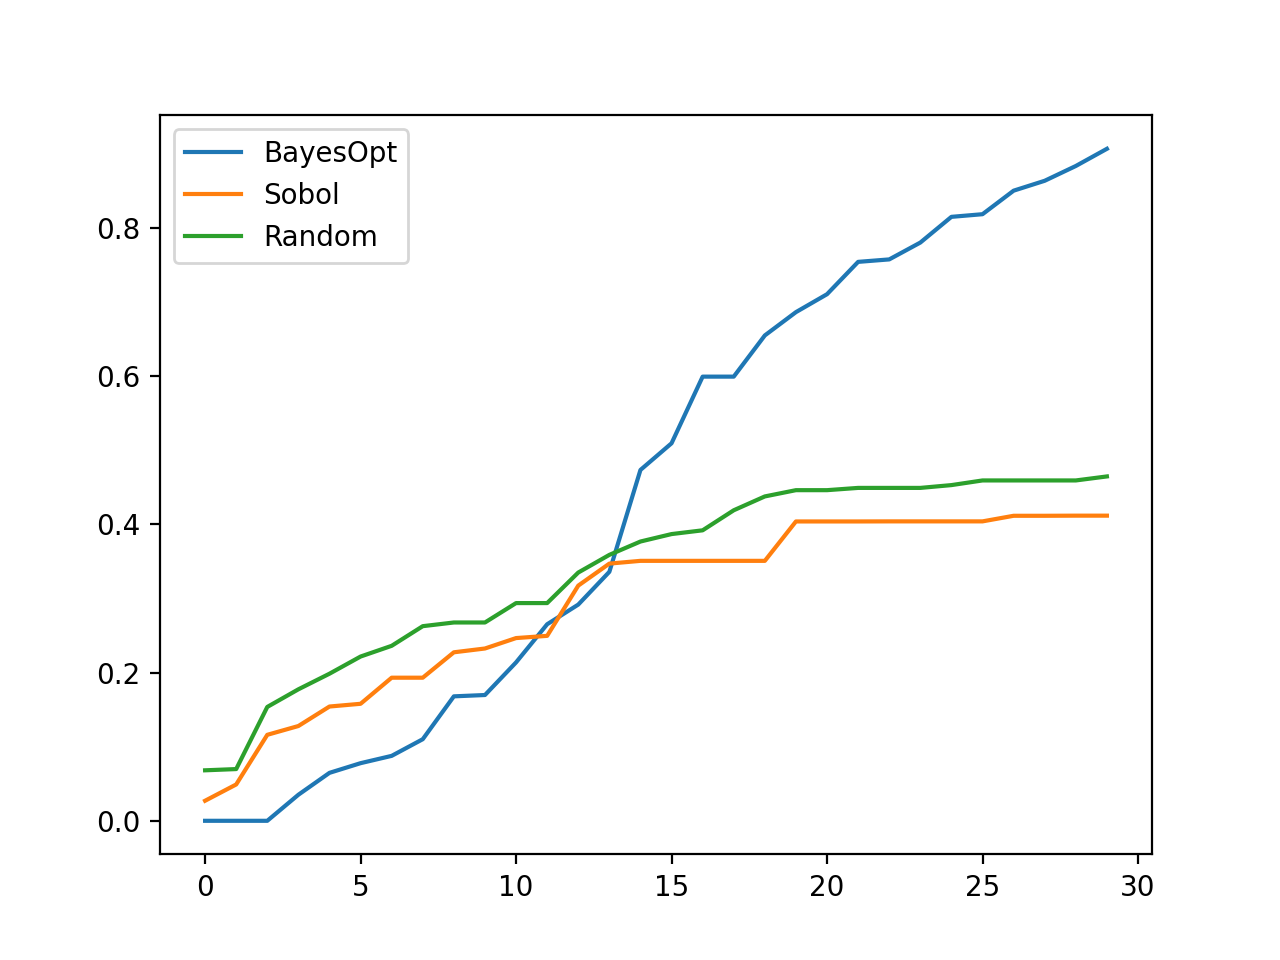
\includegraphics[height=200px]{figures/3_6.1.png}\end{align*}
\begin{align*}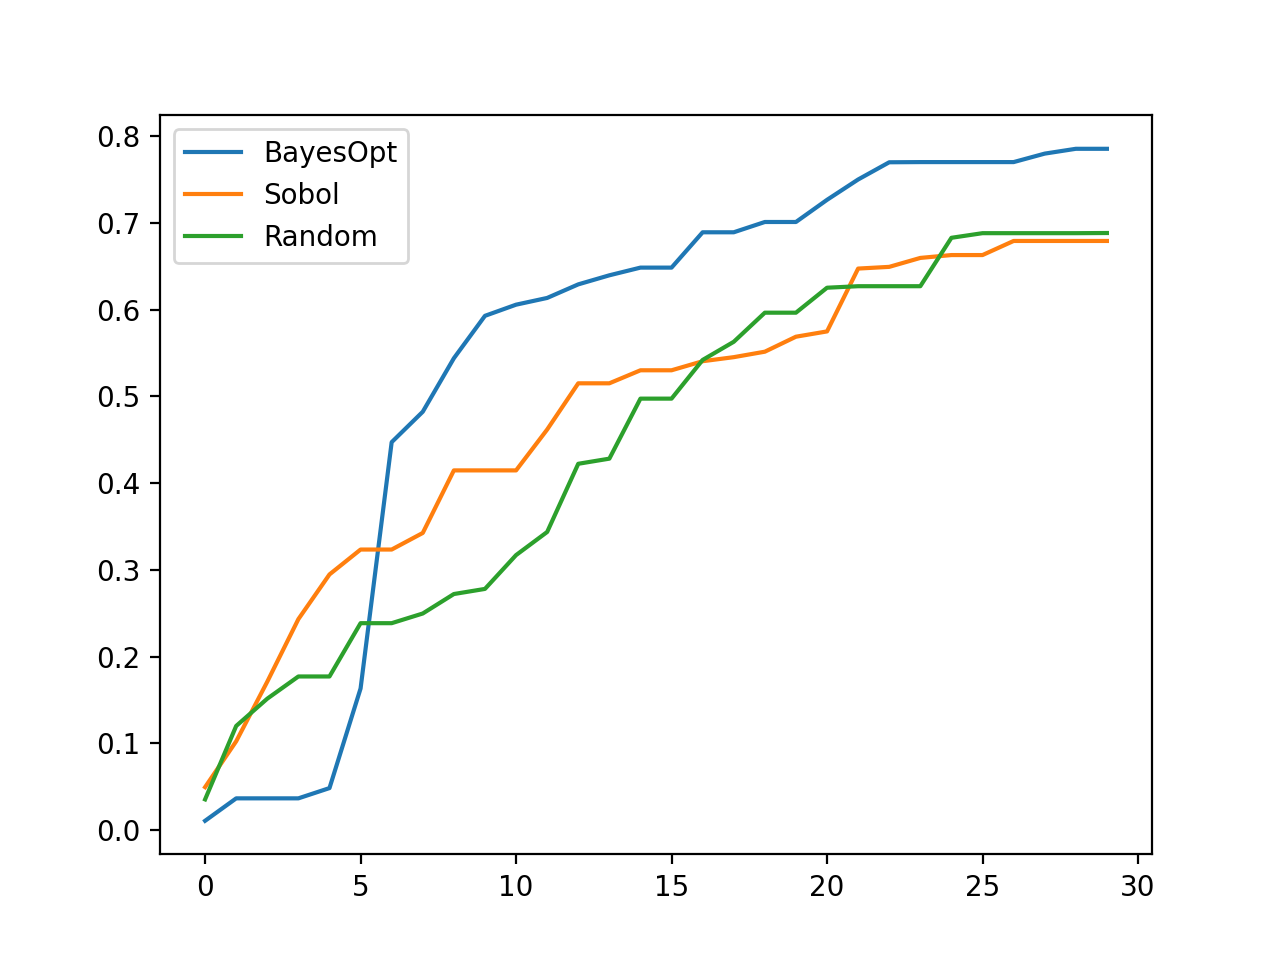
\includegraphics[height=200px]{figures/3_6.2.png}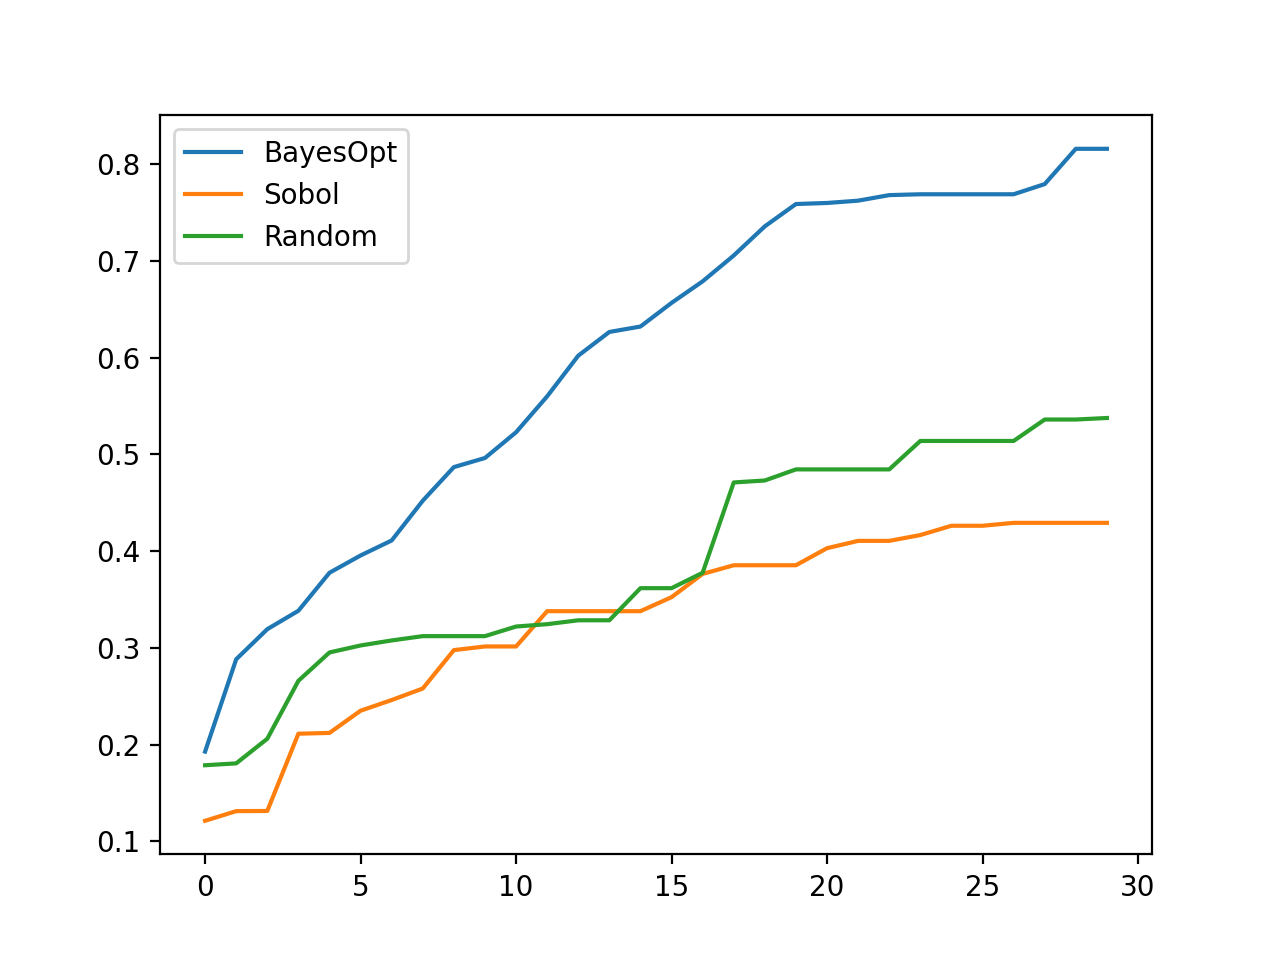
\includegraphics[height=200px]{figures/3_6.3.png}\end{align*}

\subsection*{7}
Here are the learning curves and the p-values for the three problems (six-hump, LDA, SVM respectively) by the average gap over $20$ experiments against the number of new observations, up to $150$ iterations. \\
One observations is that, for the two discrete domain, the random search works surprisingly well: since there are $288$ points in the LDA domain, so, there is a probability of $1-\left(\frac{287}{288}\right)^150=0.4065$ to have the optimal points being sampled over the $150$ uniform samples across the domain. We have $2800$ points in the SVM domain, and that is why from the latter two figures, we can see that the gap of the randomized search and the p-value are catching up quicker in LDA than SVM. 

\begin{align*}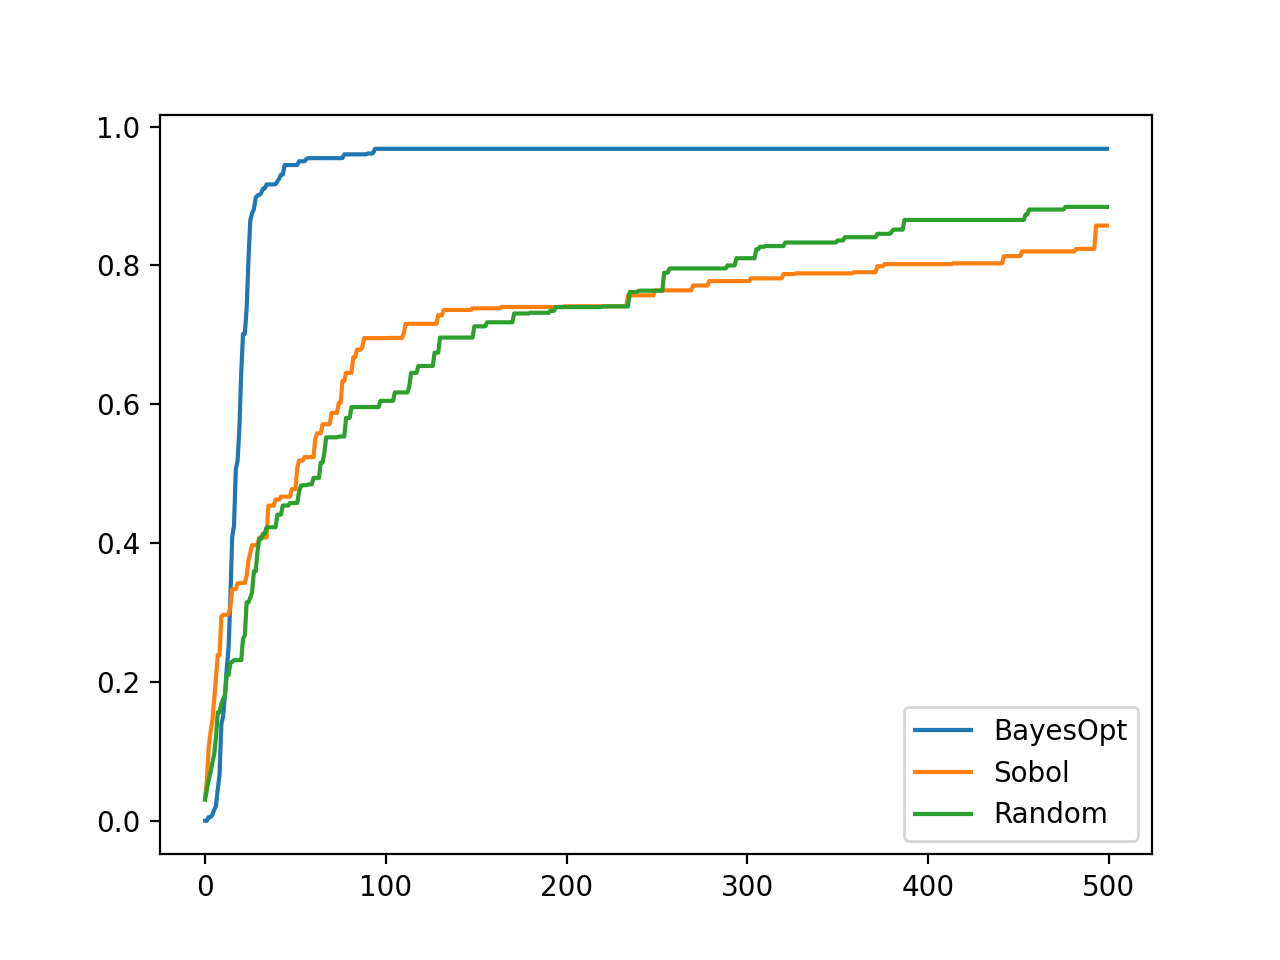
\includegraphics[height=200px]{figures/3_7.1.png}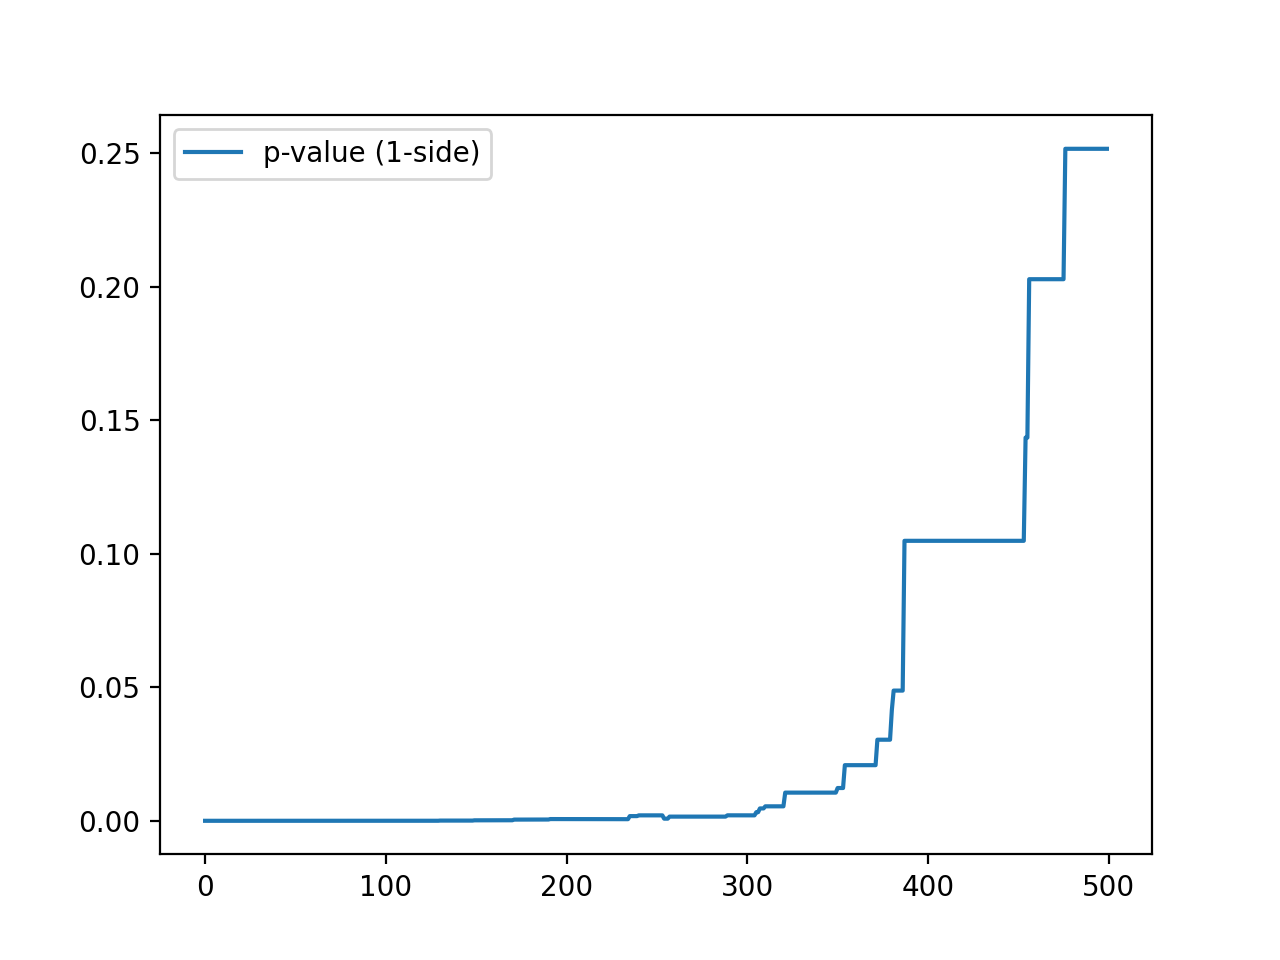
\includegraphics[height=200px]{figures/3_7.1'.png}\end{align*}
\begin{align*}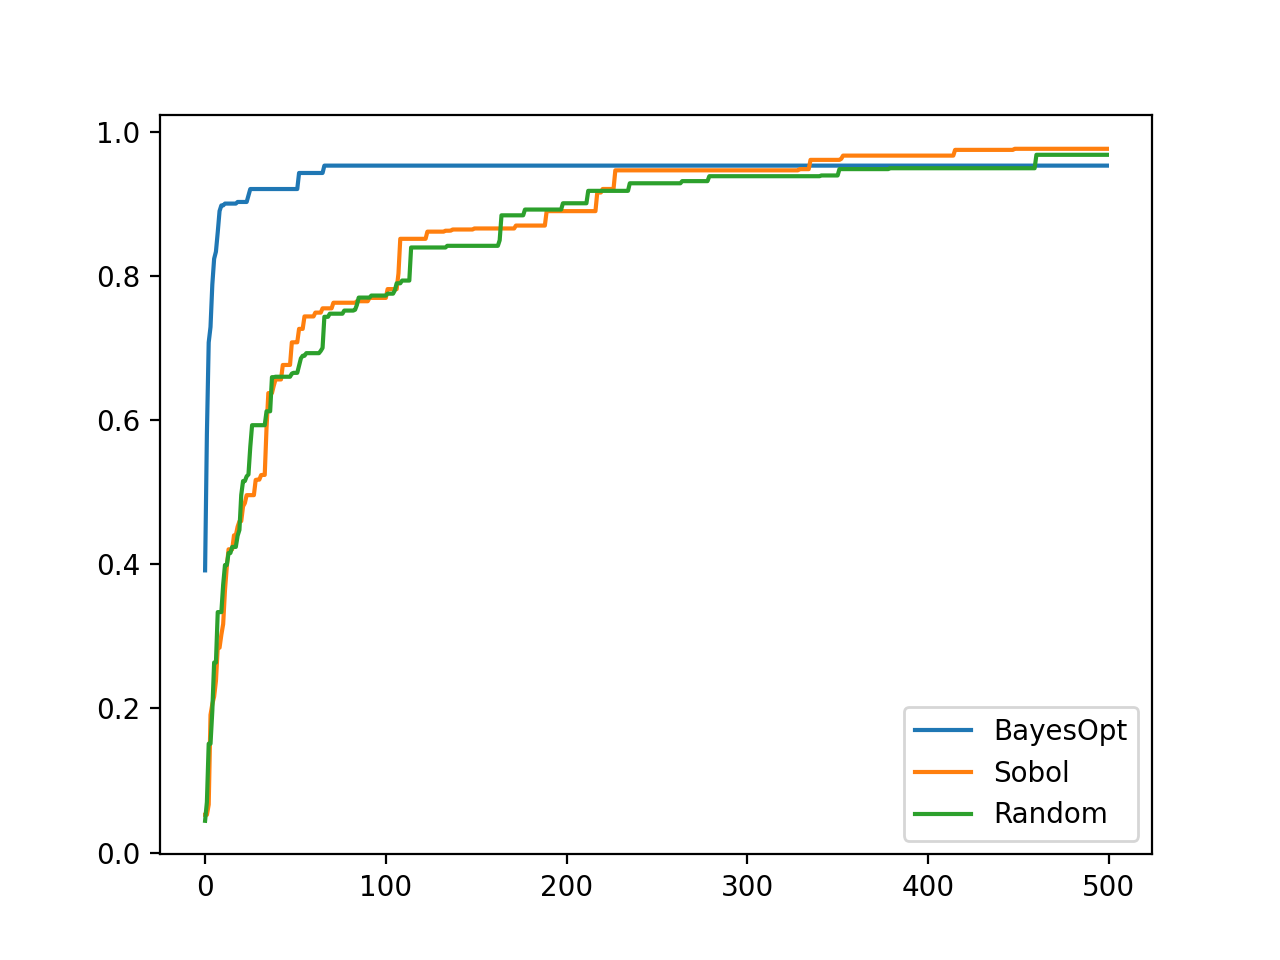
\includegraphics[height=200px]{figures/3_7.2.png}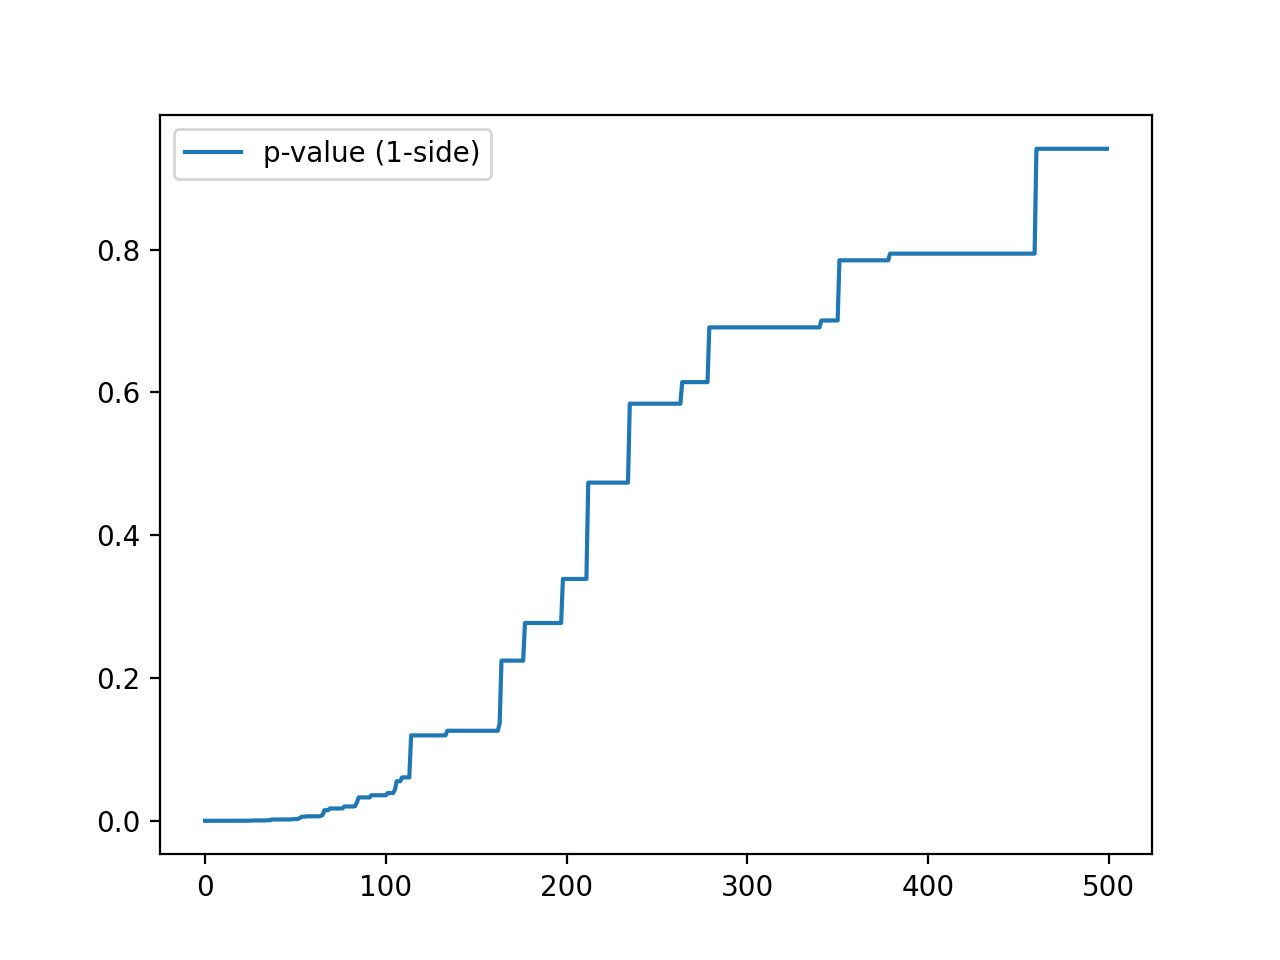
\includegraphics[height=200px]{figures/3_7.2'.png}\end{align*}
\begin{align*}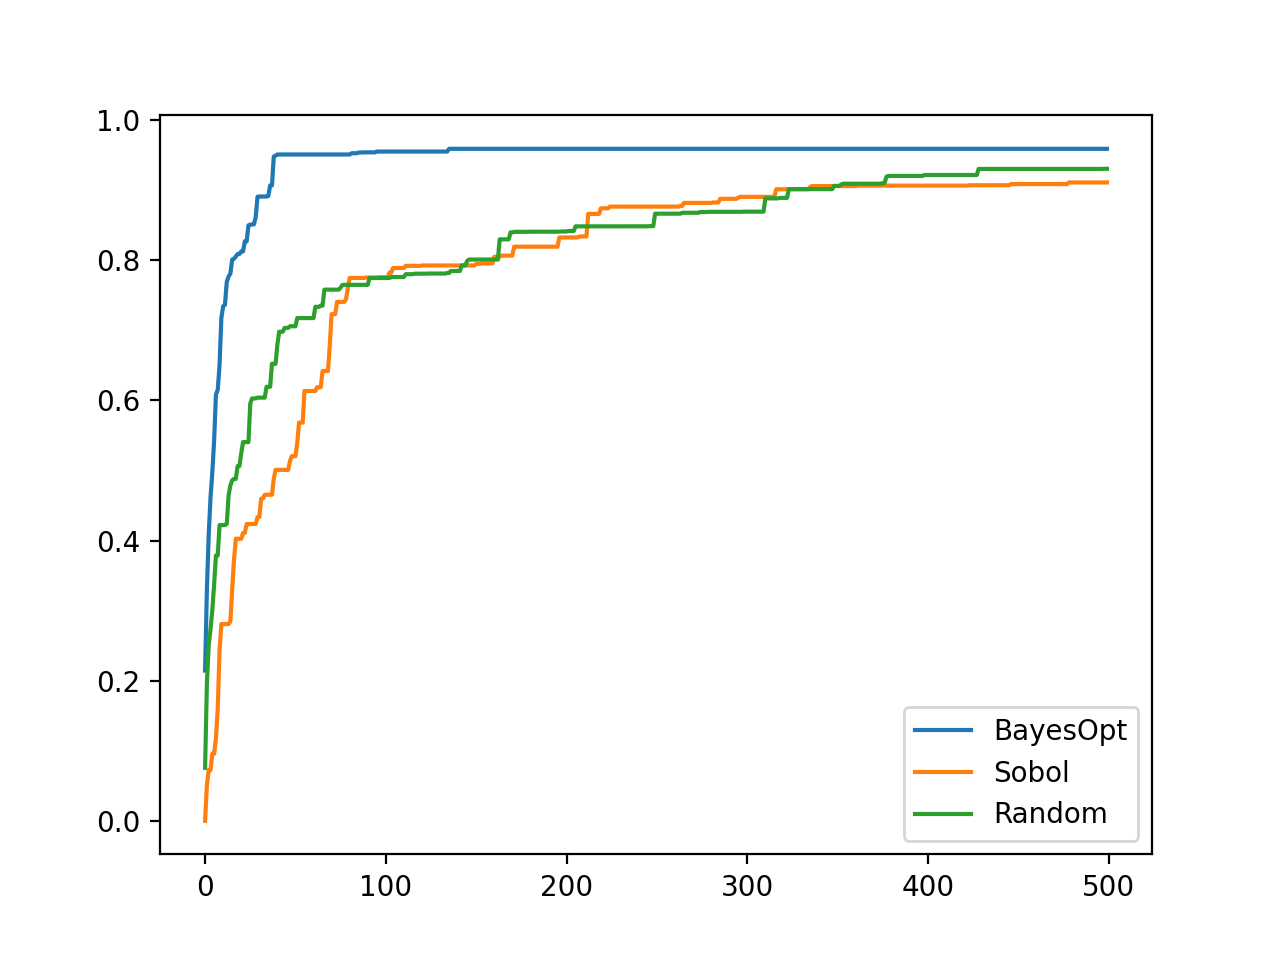
\includegraphics[height=200px]{figures/3_7.3.png}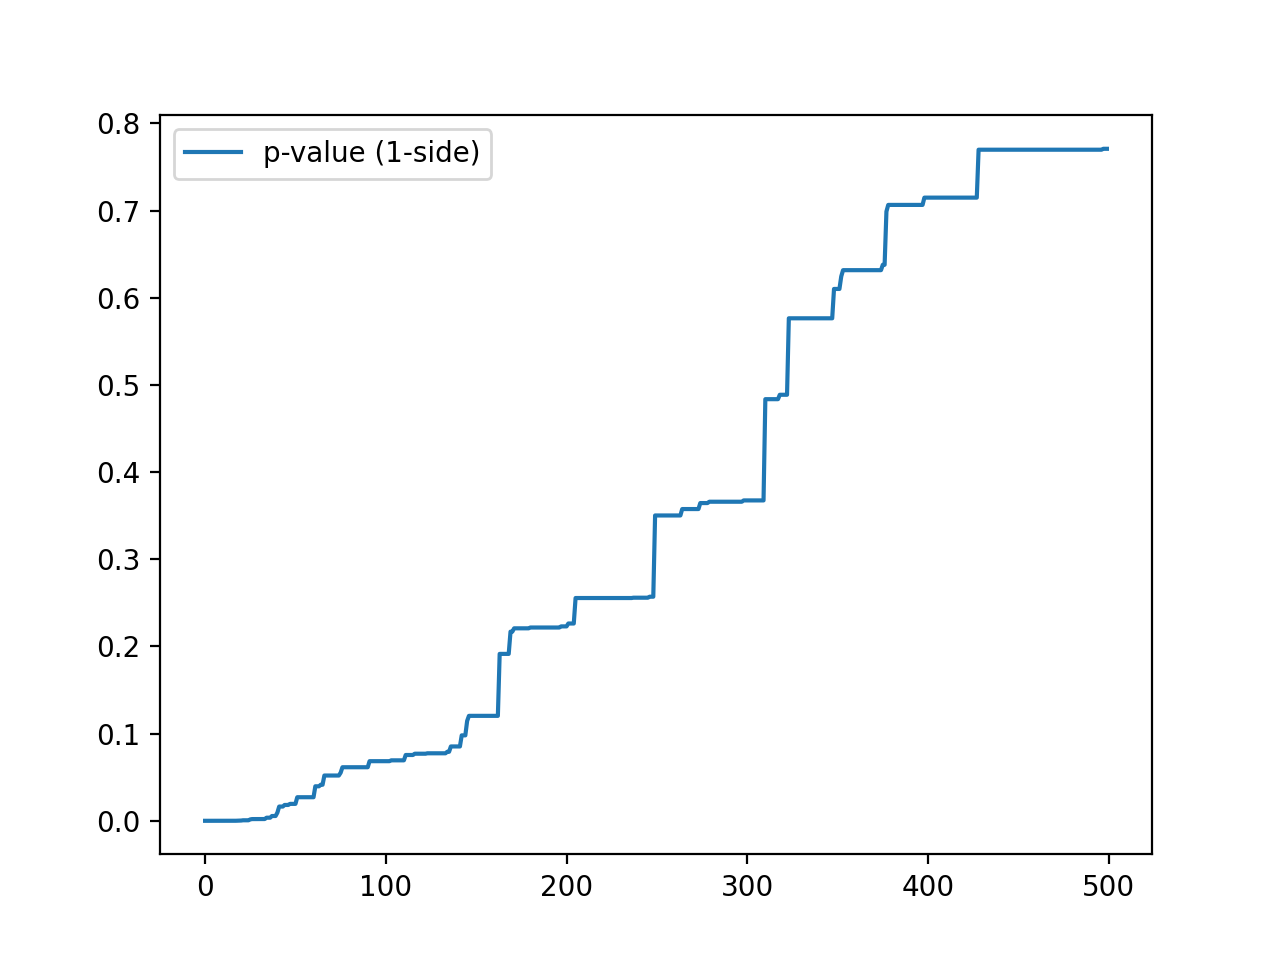
\includegraphics[height=200px]{figures/3_7.3'.png}\end{align*}

From the figures, we can clearly see that the Bayesian optimization method is much better than both the random and the Sobol sequence search. In particular, the gap of Bayesian method converges to $1$ soon after $40$ observations. And the $p$-value drops dramatically after about $10$ observations. Similar trend is found in the other two datasets (LDA and SVM), but not as significant, due to the small domain size as discussed above.

Specifically, the result of the gap values and the $p$-value for the paired t-tests are summarized below\footnote{Due to a mistake in the code, exact data are lost, indicated as $*$. Approximate values can be found on the figures above} (six-hump, LDA, SVM respectively).\\

\begin{center}
\begin{tabular}{|c|c|c|c|}
\hline
\# observations & gap (EI) & gap (random) & p-value \\
\hline
 $30$ & $0.9009$ & $0.3979$ & $*$ \\
\hline
 $60$ & $0.9545$ & $0.5239$ & $*$ \\
\hline
 $90$ & $0.9600$ & $0.6952$ & $*$ \\
\hline
$120$ & $0.9680$ & $0.7158$ & $*$ \\
\hline
$150$ & $0.9680$ & $0.7382$ & $*$ \\
\hline
\end{tabular}
\end{center}

\begin{center}
\begin{tabular}{|c|c|c|c|}
\hline
\# observations & gap (EI) & gap (random) & p-value \\
\hline
 $30$ & $0.9204$ & $0.5172$ & $*$ \\
\hline
 $60$ & $0.9426$ & $0.7436$ & $*$ \\
\hline
 $90$ & $0.9528$ & $0.7647$ & $*$ \\
\hline
$120$ & $0.9528$ & $0.8513$ & $*$ \\
\hline
$150$ & $0.9528$ & $0.8656$ & $*$ \\
\hline
\end{tabular}
\end{center}

\begin{center}
\begin{tabular}{|c|c|c|c|}
\hline
\# observations & gap (EI) & gap (random) & p-value \\
\hline
 $30$ & $0.8908$ & $0.4335$ & $0.0020$ \\
\hline
 $60$ & $0.9511$ & $0.6136$ & $0.0270$ \\
\hline
 $90$ & $0.9541$ & $0.7755$ & $0.0614$ \\
\hline
$120$ & $0.9553$ & $0.7921$ & $0.0770$ \\
\hline
$150$ & $0.9593$ & $0.7927$ & $0.1204$ \\
\hline
\end{tabular}
\end{center}

In terms of the iterations $n$ it requires to have the $p$-value larger than $0.05$, when comparing $n$ rounds of random samples against $30$ rounds of observations using Bayesian optimization, we have the following results:

\begin{center}
\begin{tabular}{|c|c|c|c|}
\hline
Policy & Six-hump & LDA & SVM \\
\hline
Iterations & $\sim370$ & $\sim90$ & $\sim60$ \\
\hline
\end{tabular}
\end{center}

So, from the above experiments, we can conclude that the Bayesian optimization might start as slow as random search for the first few ($\sim10$) observations, and then, it speeds up greatly and converges to the optimal significantly quickly at around $40$ observations. Then, as more observations is picked, the randomized searches started to catch up with on the gap, when Bayesian optimization could not make too much meaningful improvements at this point (the optimal are too close to observed points that EI vanishes). Eventually, both policy would all converge to the optimum.

\newpage
\section{Bonus 1}
\subsection{Setup}
For the first bonus section, we will investigate the effect of `real-time' hyperparameters-tuning on the mean gap. Specifically, we will set up the experiment as follows.

\begin{itemize}
	\item[0)] define the negated six-hump function after the logarithmic transformation proposed in the previous part;
	\item[1)] sample from the domain a Sobol sequence of length $5$ as the prior knowledge of the function;
	\item[2)] create three parallel Gaussian process, all of which use constant $\mu=0$ mean function, and square-exponential covariance kernel with default $0.6931$ for the two dimension of the lengthscale and the output scale, denoted as $GP_1$, $GP_2$, $GP_3$;
	\item[3)] 
	\textbullet\ Do not tune the hyperparameters for $GP_1$;\\
	\textbullet\ Tune the hyperparameters for $GP_2$ only with the $5$ common prior samples, i.e., by maximizing marginal log-likelihood;\\
	\textbullet\ Tune the hyperparameters for $GP_3$ with the $5$ common prior samples and throughout the optimization process with all the observed samples, i.e., by maximizing marginal log-likelihood;
	\item[4)] Use randomized search as baseline performance;
	\item[5)] Repeat (1) - (3) $20$ times, plot the average gap for the four methods, calculate the p-value for a paired one-sided t-test for the hypothesis that the $GP_3$ performs better than $GP_1$ and $GP_2$.  
\end{itemize}

\subsection{Result}
\begin{align*}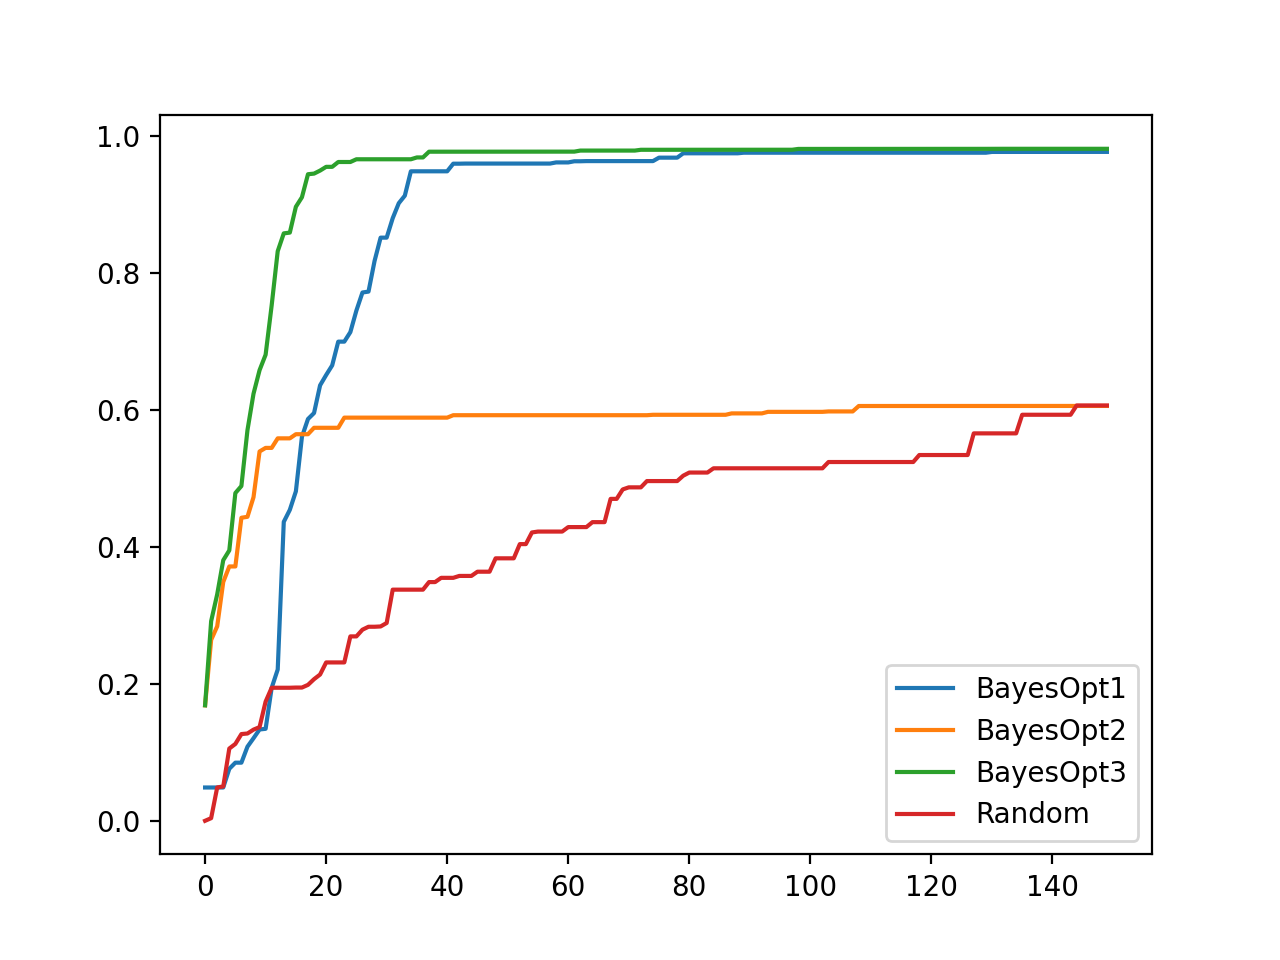
\includegraphics[height=200px]{figures/4_1.png}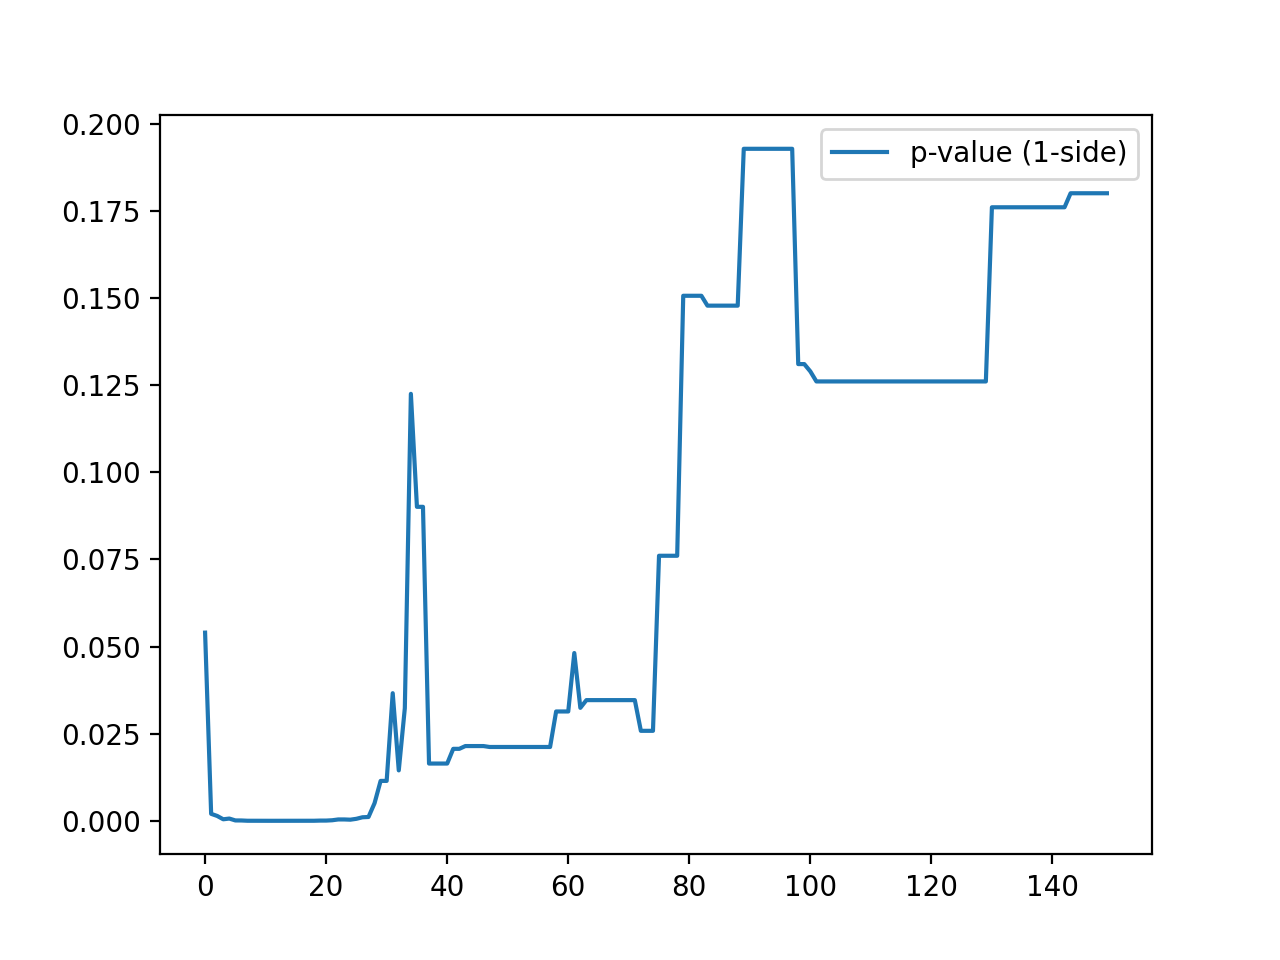
\includegraphics[height=200px]{figures/4_1'.png}\end{align*}

\subsection{Conclusion}
As we can see from the figure on the left, it is clear that the $GP2$ method is not nearly as great as the other two algorithms overall. However, during the beginning part of the process, since both $GP_2$ and $GP_3$ are tuned exactly the same, they perform similarly. As we observe more samples, since we only have $5$ prior samples for tuning $GP_2$, it has a high chance that the points does not represents the function nicely, leading to a low accuracy (probability due to underfitting), even after we condition on the new observations. So, the $p$-value for $GP_3$ better than $GP_2$ is not included.\\
The comparison for the $GP_1$ and $GP_2$ is also interesting. Clearly, the $GP_3$ (where we constantly tune the hyperparameters) converges much faster to the global maximum than the $GP_1$, which uses default hyperparameters. However, the $GP_1$ model would catch up with $GP_2$ after $20$ iterations, and performs approximately as good as $GP_3$ after $40$ iterations. And after $80$ iterations, there is no statistical evidence at $p=0.05$ level to say that $GP_3$ performs better than $GP_1$.

\newpage
\section{Bonus 2}
\subsection{Setup}
We have compared the performance of random search over $n$ iterations versus the performance of Bayesian optimization over $30$ rounds, and it seems that with randomized search would requires a few times more iterations to reach the same level. But, what if we are comparing those two methods over the same number of iterations? \\
So, with the same setup as before, only one change that we using paired t-tests on gap over the same number of iterations.

\subsection{Result}
\begin{align*}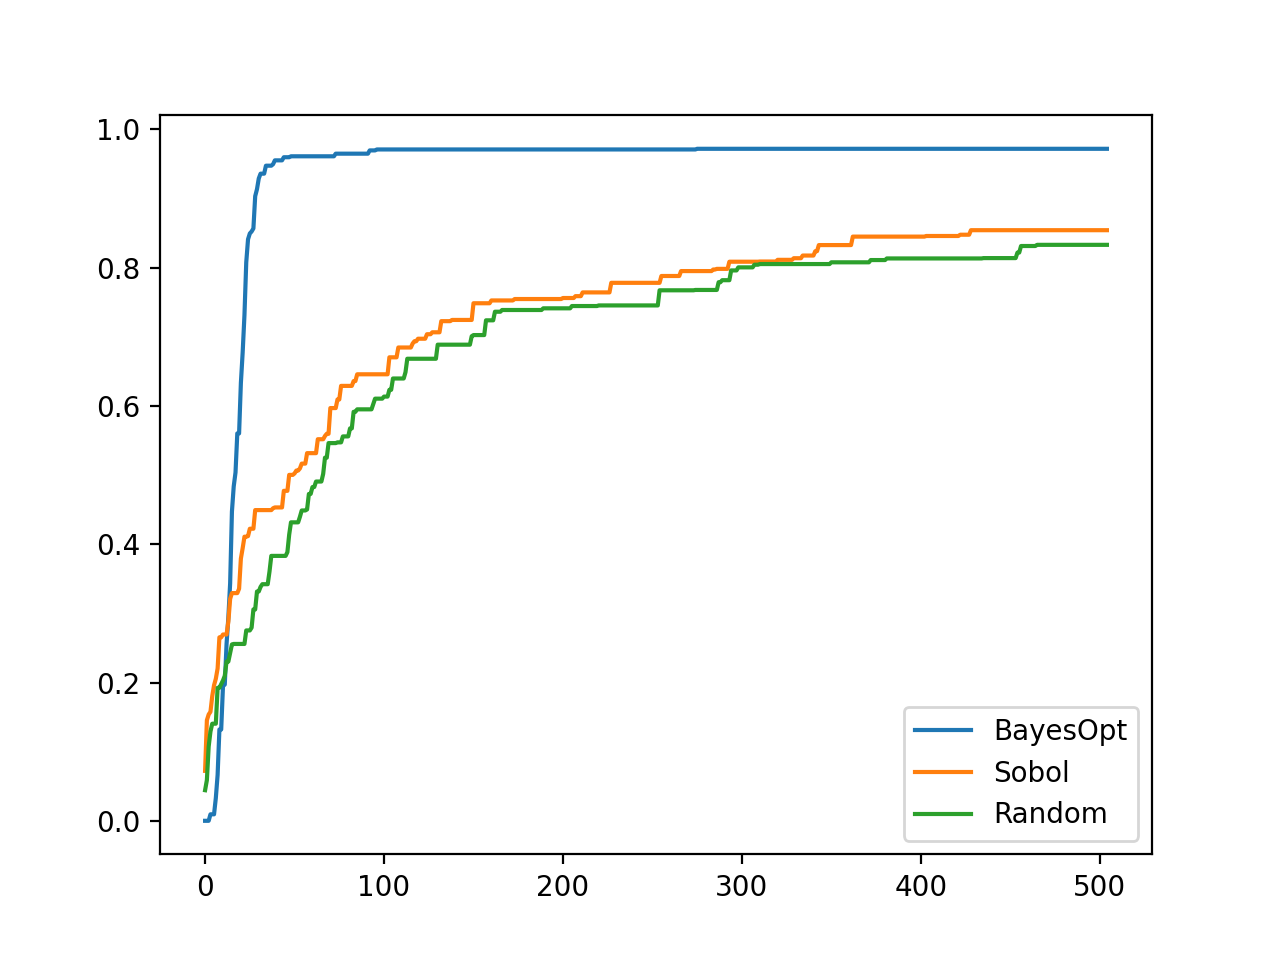
\includegraphics[height=200px]{figures/4_2.1.png}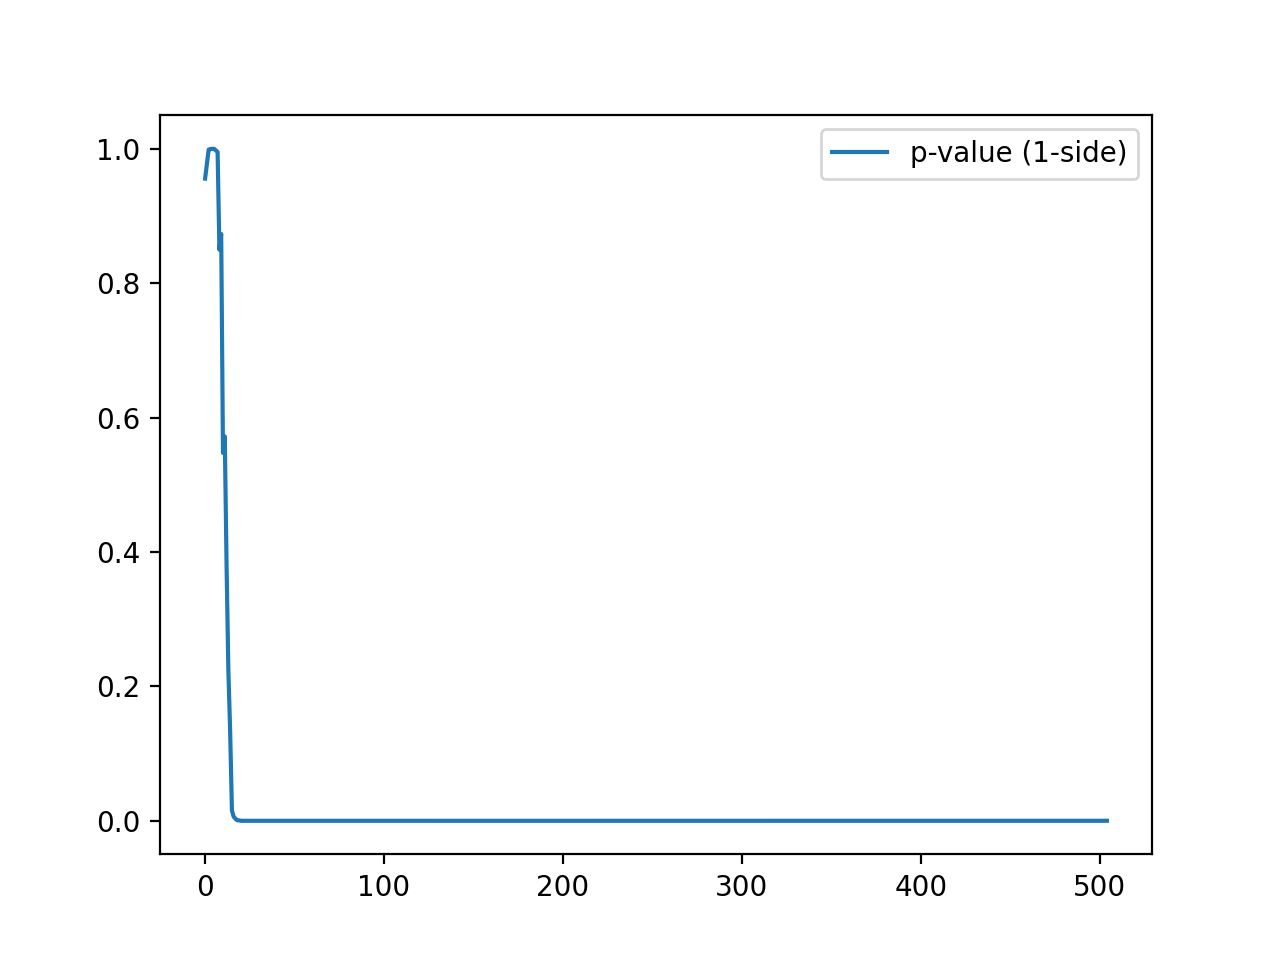
\includegraphics[height=200px]{figures/4_2.1'.png}\end{align*}
\begin{align*}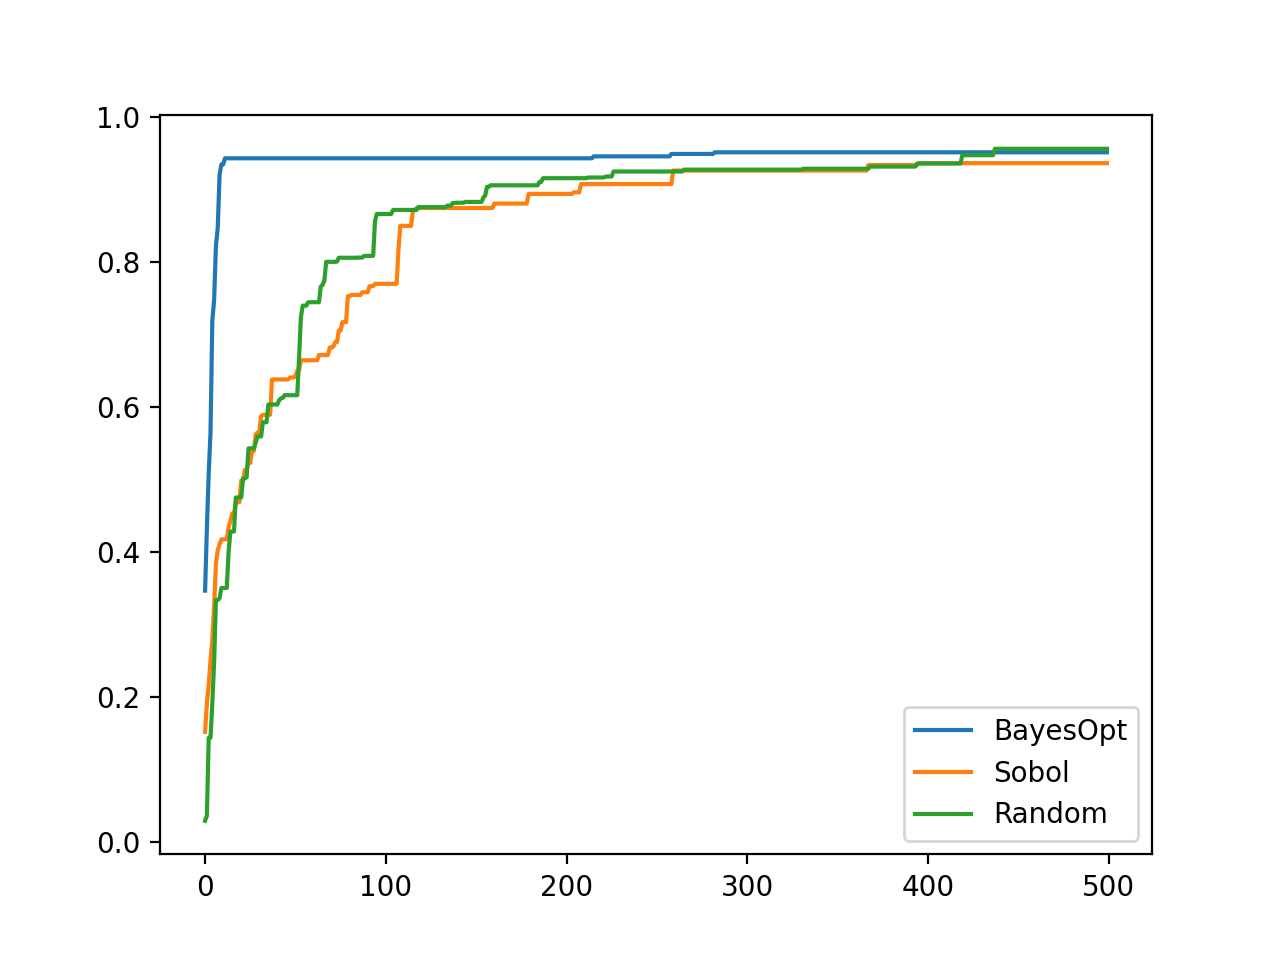
\includegraphics[height=200px]{figures/4_2.2.png}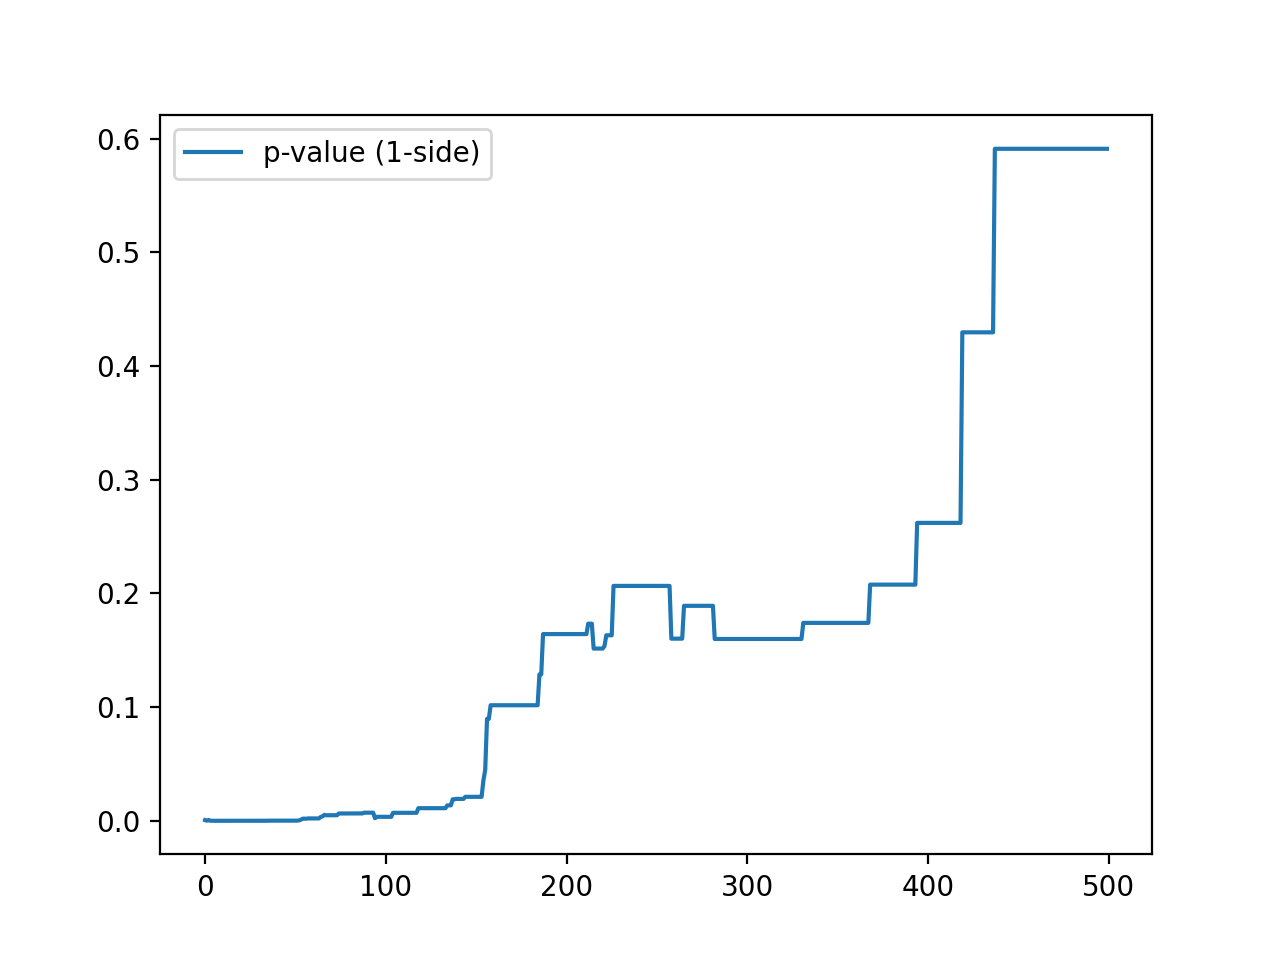
\includegraphics[height=200px]{figures/4_2.2'.png}\end{align*}
\begin{align*}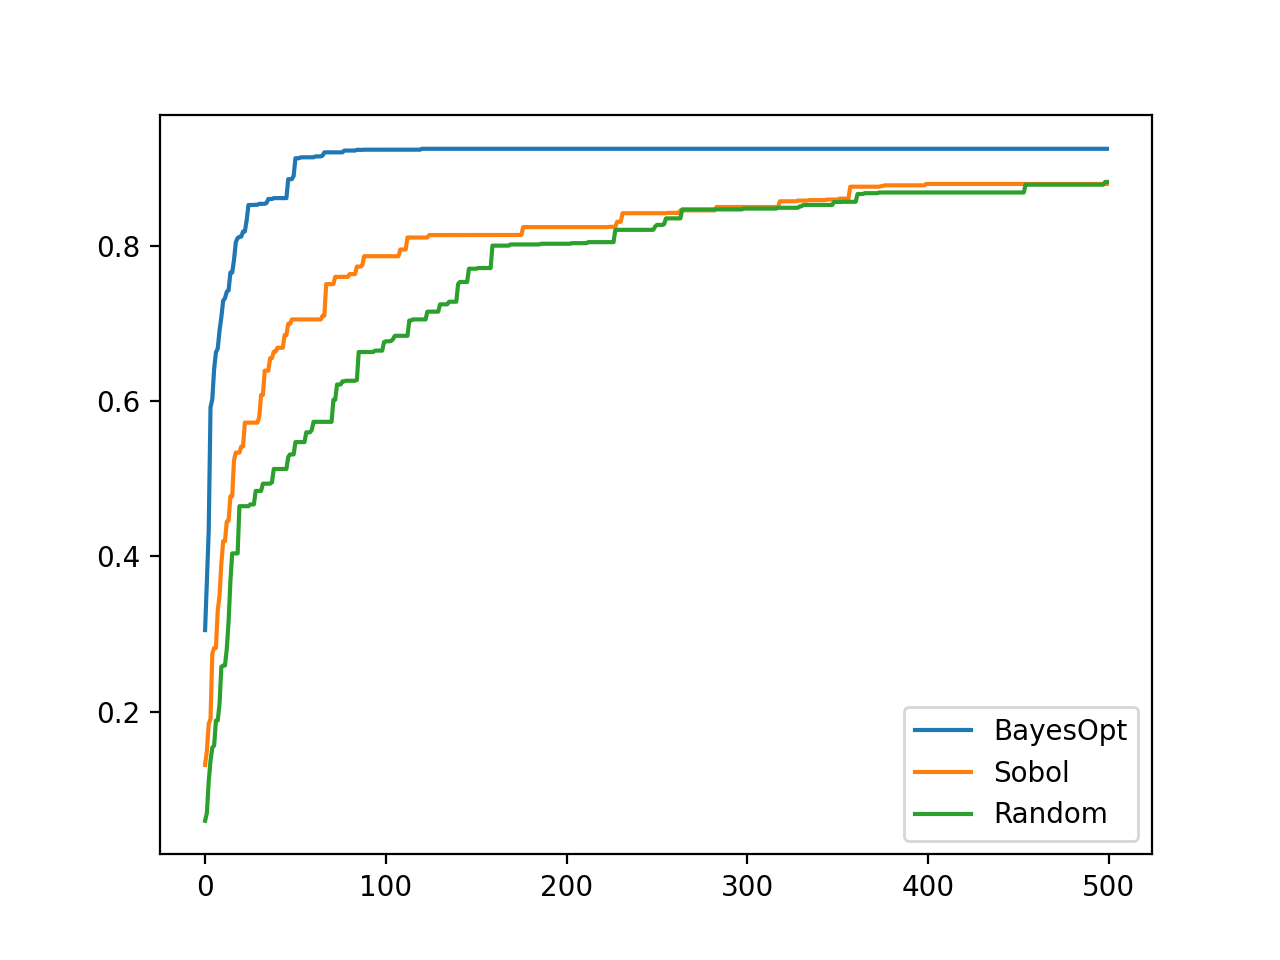
\includegraphics[height=200px]{figures/4_2.3.png}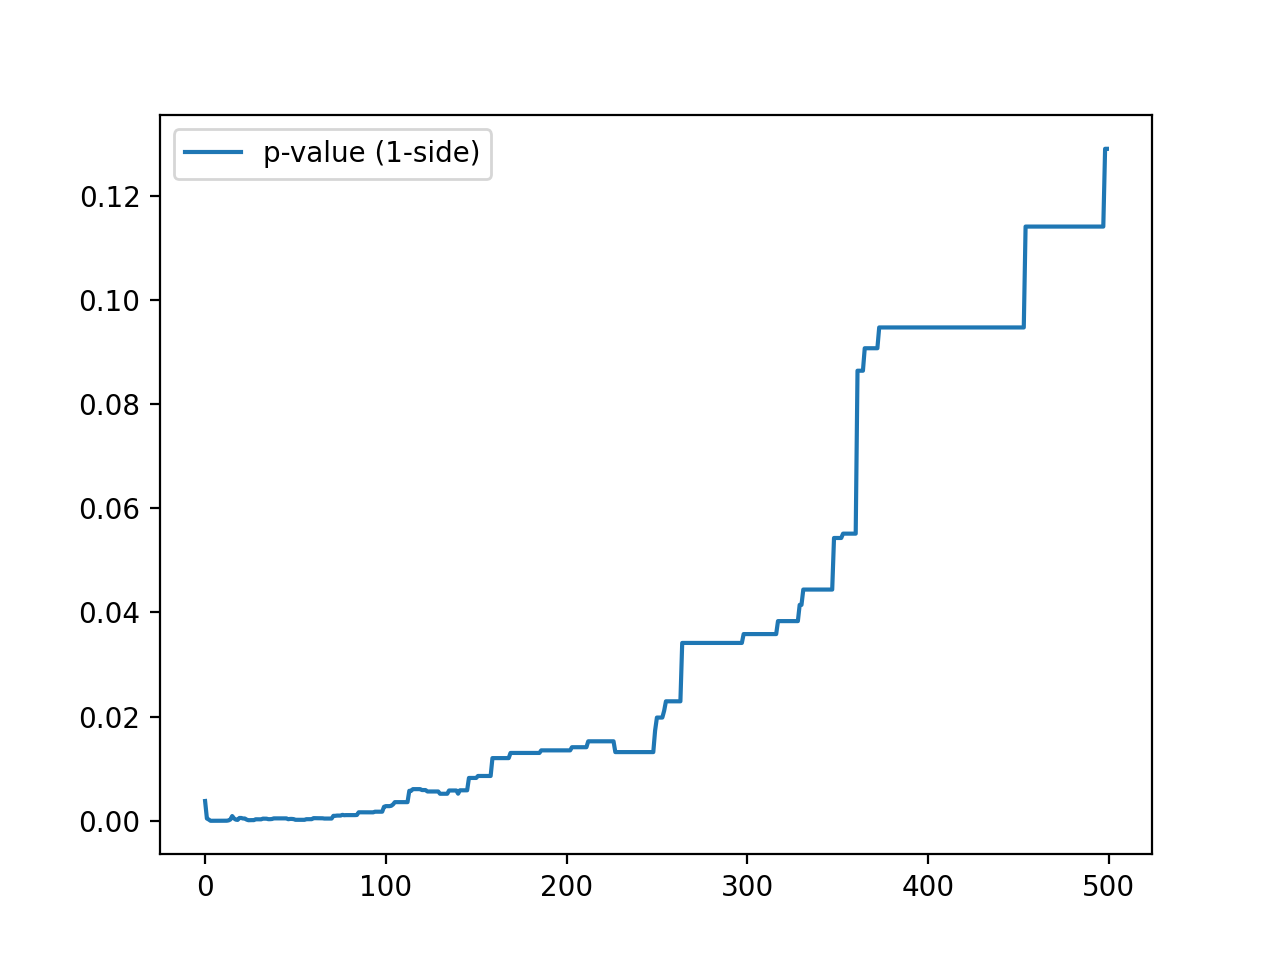
\includegraphics[height=200px]{figures/4_2.3'.png}\end{align*}

\begin{center}
\begin{tabular}{|c|c|c|c|}
\hline
\# observations & gap (EI) & gap (random) & $p$-value \\
\hline
 $30$ & $0.8543$ & $0.2697$ & $1\times10^{-6}$ \\
\hline
 $60$ & $0.9149$ & $0.4083$ & $1\times10^{-5}$ \\
\hline
 $90$ & $0.9194$ & $0.4956$ & $1\times10^{-4}$ \\
\hline
$120$ & $0.9292$ & $0.5284$ & $1\times10^{-2}$ \\
\hline
$150$ & $0.9301$ & $0.6027$ & $1\times10^{-2}$ \\
\hline
\end{tabular}
\end{center}

\begin{center}
\begin{tabular}{|c|c|c|c|}
\hline
\# observations & gap (EI) & gap (random) & p-value \\
\hline
 $30$ & $0.9847$ & $0.5063$ & $1\times10^{-5}$ \\
\hline
 $60$ & $0.9847$ & $0.6389$ & $0.0001$ \\
\hline
 $90$ & $0.9847$ & $0.6891$ & $0.0003$ \\
\hline
$120$ & $0.9847$ & $0.6996$ & $0.0004$ \\
\hline
$150$ & $0.9847$ & $0.7273$ & $0.0010$ \\
\hline
\end{tabular}
\end{center}

\begin{center}
\begin{tabular}{|c|c|c|c|}
\hline
\# observations & gap (EI) & gap (random) & p-value \\
\hline
 $30$ & $0.8675$ & $0.5795$ & $0.0017$ \\
\hline
 $60$ & $0.9648$ & $0.7384$ & $0.0004$ \\
\hline
 $90$ & $0.9679$ & $0.8058$ & $0.0006$ \\
\hline
$120$ & $0.9690$ & $0.8446$ & $0.0005$ \\
\hline
$150$ & $0.9690$ & $0.8530$ & $0.0005$ \\
\hline
\end{tabular}
\end{center}

\begin{center}
\begin{tabular}{|c|c|c|c|}
\hline
Policy & Six-hump & LDA & SVM \\
\hline
Iterations & $\geq500$ & $\sim165$ & $\sim360$ \\
\hline
\end{tabular}
\end{center}

\subsection{Conclusion}
As we would have imagined, for the discrete domain (LDA and SVM in this case) with less elements, after certain iterations, the random search would do as good as the Bayesian optimization and there would be no statistical significance that Bayesian optimization would be still better. However, for the six-hump function, since the domain is continuous (grid of $1000\times1000$ for maximizing EI), the randomized algorithm is having a hard time finding the optimal locations. \\
However, this can also guide when to terminate the optimization. In particular, for a discrete domain, we can explicitly calculate the required number of iterations using the $PAC$ model and use it as a hard upper bound to terminate the optimization procedure. However, we would still hope that there are other termination conditions and such hard upper bound would never be met.

\newpage

\section{Code}
The code and all related files are uploaded to the Github at \url{https://github.com/TimDSF/BayesianOptimization/tree/main/CSE544_Project_TimDong/source}.

\section{References}
\nocite{*}
\bibliography{References}
\bibliographystyle{IEEEtranN}

\end{document}
